\documentclass[preprint2]{aastex62}
\graphicspath{ {./figs/} }
\usepackage{xspace, url, amsmath}
%%
\newcommand{\z}[1]{$z \sim {#1}$}
\newcommand{\FSPS}{{\sc FSPS}\xspace}
\newcommand{\pFSPS}{{\tt \textbf{python-fsps}}\xspace}
\newcommand{\CloudyFSPS}{{\tt \textbf{CloudyFSPS}}\xspace}
\newcommand{\Mappings}{{\sc Mappings-III}\xspace}
\newcommand{\Pegase}{\textsc{P{\'e}gase}\xspace}
\newcommand{\SB}{\textsc{Starburst-99}\xspace}
\newcommand{\Popstar}{\textsc{PopStar}\xspace}
\newcommand{\Cloudy}{\textsc{Cloudy}\xspace}
\newcommand{\Prospector}{{\sc Prospector}\xspace}
\newcommand{\hii}{H\,{\sc ii}\xspace}
\newcommand{\nii}{[N\,{\sc ii}]\xspace}
\newcommand{\niii}{[N\,{\sc iii}]\xspace}
\newcommand{\sii}{[S\,{\sc ii}]\xspace}
\newcommand{\siii}{[S\,{\sc iii}]\xspace}
\newcommand{\oiii}{[O\,{\sc iii}]\xspace}
\newcommand{\oii}{[O\,{\sc ii}]\xspace}
\newcommand{\oi}{[O\,{\sc i}]\xspace}
\newcommand{\neiii}{[Ne\,{\sc iii}]\xspace}
\newcommand{\heii}{[He\,{\sc ii}]\xspace}
\newcommand{\hei}{[He\,{\sc i}]\xspace}
\newcommand{\civ}{C\,{\sc iv}\xspace}
\newcommand{\SiuII}{[Si\,{\sc ii}]\xspace}
\newcommand{\SiuIII}{[Si\,{\sc iii}]\xspace}
\newcommand{\alII}{[Al\,{\sc ii}]\xspace}
\newcommand{\mgii}{[Mg\,{\sc ii}]\xspace}
\newcommand{\ciii}{C\,{\sc iii}]\xspace}
\newcommand{\cii}{[C\,{\sc ii}]\xspace}
\newcommand\vs{\ensuremath{\mathrm{vs.}}\xspace}
\newcommand{\sigmaL}{\ensuremath{\sigma_{\mathrm{line}}}\xspace}
\newcommand{\sigmaR}{\ensuremath{\sigma_{\mathrm{ratio}}}\xspace}
\newcommand{\sigmaRU}{\ensuremath{\sigma_{\mathrm{ratio,}\,\mathcal{U}}}\xspace}
\newcommand{\sigmaRZ}{\ensuremath{\sigma_{\mathrm{ratio,}\,Z}}\xspace}
\newcommand{\sigmaU}{\ensuremath{\sigma_{\mathcal{U}}}\xspace}
\newcommand{\sigmaZ}{\ensuremath{\sigma_{Z}}\xspace}
\newcommand{\femline}{\ensuremath{f_{\mathrm{line}}}\xspace}
\newcommand\Lsun{\ensuremath{\mathrm{L_{\sun}}}\xspace}
\newcommand\Msun{\ensuremath{\mathrm{M_{\sun}}}\xspace}
\newcommand{\ha}{\ensuremath{\mathrm{H\alpha}}\xspace}
\newcommand{\hb}{\ensuremath{\mathrm{H\beta}}\xspace}
\newcommand{\Myr}{$\,$Myr\xspace}
\newcommand{\logten}{\ensuremath{\log_{10}}}
\newcommand{\logZ}{\ensuremath{\logten \mathrm{Z}/\mathrm{Z}_{\sun}}\xspace}
\newcommand{\logOH}{\ensuremath{\logten (\mathrm{O}/\mathrm{H})}\xspace}
\newcommand{\logZeq}[1]{\ensuremath{\logten \mathrm{Z}/\mathrm{Z}_{\sun} = #1}}
\newcommand{\ang}{\ensuremath{\mbox{\AA}}\xspace}
\newcommand{\logQ}[1]{\ensuremath{\logten Q_{#1}}}
\newcommand{\QH}{\ensuremath{Q_{\mathrm{H}}}}
\newcommand{\QHat}{\ensuremath{\hat{Q}_{\mathrm{H}}}}
\newcommand{\U}{\ensuremath{\mathcal{U}_{0}}\xspace}
\newcommand{\logU}{\ensuremath{\logten \mathcal{U}_0}}
\newcommand{\logUeq}[1]{\ensuremath{\logten \mathcal{U}_0 = #1}}
\newcommand{\kms}{\ensuremath{\;\mathrm{km}\;\mathrm{s}^{-1}}\xspace}
\newcommand{\fcont}{\ensuremath{\mathcal{F}_{\mathrm{cont}}(\lambda)}\xspace}
\newcommand{\fline}{\ensuremath{\mathcal{F}_{\mathrm{line}}(\lambda)}\xspace}
\newcommand{\mage}{{\sc Meg}a{\sc S}a{\sc ura}\xspace}
\newcommand{\Te}{\ensuremath{T_{\mathrm{e}}}\xspace}
\newcommand{\XXX}{{\bf \color{red}{XXX} }}
%\newcommand{\XXX}[1]{\colorbox{red}{#1}}
%%
\newcommand{\vdag}{(v)^\dagger}
\newcommand\aastex{AAS\TeX}
\newcommand\latex{La\TeX}
%%%%%%%%%%%%%%%%%%%%%%%%%%%%%%%%%%%%%%%%%%%%%%%%%%%%%%%%%%%%%%%%%%%%%%%%%%%%%%%%
%%
%\received{July 1, 2016}
\revised{\today}
%\accepted{\today}
%\submitjournal{ApJ}
%%
\shorttitle{}
\shortauthors{Byler et al.}
%%
%%%%%%%%%%%%%%%%%%%%%%%%%%%%%%%%%%%%%%%%%%%%%%%%%%%%%%%%%%%%%%%%%%%%%%%%%%%%%%%%
\begin{document}
\title{UV and optical metallicities in local and high-redshift star-forming galaxies}
%%%%%%%%%%%%%%%%%%%%%%%%%%%%%%%%%%%%%%%%%%%%%%%%%%%%%%%%%%%%%%%%%%%%%%%%%%%%%%%%
%%
\correspondingauthor{Nell Byler}
\email{nell.byler@anu.edu.au}
%%
\author[0000-0002-7392-3637]{Nell Byler}
\affil{Research School of Astronomy and Astrophysics, The Australian National University, ACT, Australia}
\affil{ARC Centre of Excellence for All Sky Astrophysics in 3 Dimensions (ASTRO 3D), Australia}
%%
\author[0000-0001-8152-3943]{Lisa Kewley}
\affil{Research School of Astronomy and Astrophysics, The Australian National University, ACT, Australia}
\affil{ARC Centre of Excellence for All Sky Astrophysics in 3 Dimensions (ASTRO 3D), Australia}
%%
\author[0000-0002-7627-6551]{Jane Rigby}
\affil{Goddard Space Flight Center, 8800 Greenbelt Road, Greenbelt, MD 20771, USA}
%%
\author[0000-0003-4804-7142]{Ayan Acharyya}
\affil{Research School of Astronomy and Astrophysics, The Australian National University, ACT, Australia}

\author{others}
%%
%%%%%%%%%%%%%%%%%%%%%%%%%%%%%%%%%%%%%%%%%%%%%%%%%%%%%%%%%%%%%%%%%%%%%%%%%%%%%%%%
\begin{abstract}

Our ability to study the properties of the interstellar medium (ISM) in the earliest galaxies will rely on emission line diagnostics at rest-ultraviolet (UV) wavelengths. In this work, we identify metallicity-sensitive diagnostics in the UV and quantify the relationship between UV-derived metallicity and optical metallicity using a comparison sample that includes low and high-redshift galaxies with rest-frame UV and optical spectroscopy. We find that diagnostics using the \ciii$\lambda$1906,1909 emission lines are unreliable metallicity indicators and diagnostics using the \heii$\lambda$1640 emission line correlate poorly with optical abundances, and discuss possible explanations for the discrepant abundance determinations. We find that the most accurate and precise diagnostics use a combination of silicon, oxygen, and nitrogen lines over several ionization states, such as \SiuII$\lambda$1307/\SiuII$\lambda$1531 \vs \oiii$\lambda$1666/\SiuIII$\lambda$1883. We then use these diagnostics to estimate metallicities for galaxies without rest-optical spectra.
\end{abstract}
\keywords{galaxies:abundances --- galaxies:ISM --- galaxies:high-redshift --- ultraviolet:galaxies --- stars:massive}
%%%%%%%%%%%%%%%%%%%%%%%%%%%%%%%%%%%%%%%%%%%%%%%%%%%%%%%%%%%%%%%%%%%%%%%%%%%%%%%%

\section{Introduction} \label{sec:intro}

Studying the build-up of stellar mass and metals in galaxies over cosmic time is critical to understanding how galaxies form and evolve. Changes in mass and metallicity are intertwined through the star formation process, as gas is converted into stars and subsequently enriched within stars through nucleosynthetic processes. Some of this enriched gas is eventually expelled via stellar winds or supernovae (SNe), and returned to the interstellar medium (ISM). As star formation continues and the enrichment process repeats, the metal content of the galaxy increases.

The exact pattern of elemental abundances in a given galaxy depends on the history of star formation. In turn, the duration and efficiency of star formation will depend on the availability of gas, in addition to the temperature, density, and composition of the gas itself. Ultimately, our ability to understand the mechanisms that drive and sustain star formation rely on our ability to understand the physical properties of the ISM.

Fortunately, emission from ionized gas (nebular emission) in galaxies is easily observable as bright emission lines (i.e., hydrogen recombination transitions or the radiative de-excitation of collisionally excited metal ions). These emission lines are encoded with information about the local gas conditions, including the temperature, chemical composition, density, and ionization state. With some basic knowledge of atomic physics, ratios of these emission lines are used to extract the properties of the ISM.

Ratios emission lines that have proven to be particularly sensitive to properties like metallicity or density are called ``emission line diagnostics''. The best-known emission line diagnostics use transitions at optical wavelengths, and there is a long history of using these emission line diagnostics to constrain the physical properties of the ISM in galaxies with redshifts between $0<z<4$.

However, at redshifts above $z{\sim}5$, these well-established optical emission line diagnostics become observationally inaccessible with ground-based optical and IR facilities. To probe the physical conditions of the gas in the earliest galaxies, we must instead rely on emission line diagnostics that originate in the rest-ultraviolet (rest-UV) part of the spectrum. Like their optical counterparts, UV emission line diagnostics promise the ability to probe ISM conditions in distant galaxies with relative ease; S/N requirements for emission line ratios are much less restrictive than those needed for detailed stellar continuum analyses.

Unfortunately, the properties of both nebular and stellar emission in the UV are still not well understood. UV diagnostics are plagued by uncertainties driven by our comparative lack of UV spectroscopy; model predictions are less constrained and observational comparison samples are small. Moreover, the rest-UV spectra of star-forming galaxies have revealed complex and occasionally confusing features, including broad emission features (e.g., \heii$\lambda$1640), emission associated with stellar winds (\civ$\lambda$1550, {\sc S\,iv}$\lambda$1400), and emission from transitions with a non-stellar ionization source (e.g., continuum upscattering in Mg{\sc ii}$\lambda$2796). In many cases, these features overlap with nebular emission lines, making the interpretation of UV emission line diagnostics challenging.

Despite the challenges associated with interpreting UV emission line diagnostics, they are crucial for studying the most distant galaxies. Future surveys using the James Webb Space Telescope (JWST) will provide rest-UV spectroscopy for tens of thousands of galaxies at $z{\sim}5$ and above. For most of these galaxies, it will be impossible to obtain rest-optical spectroscopy, and our only means of understanding the gas in these objects will come from their rest-UV emission. Before we can apply UV emission line diagnostics to large samples of high redshift galaxies, we must ensure that that they can accurately predict key astrophysical parameters like the gas-phase metallicity. Moreover, to robustly compare the properties of high redshift galaxies with the results from lower redshift studies, we must ensure that predictions from UV emission line diagnostics are consistent with predictions from optical emission line diagnostics.

However, ensuring that UV and optical emission line diagnostics predict consistent metallicities is a non-trivial task on two accounts. First, the task requires a sample of galaxies with both rest-UV and rest-optical spectroscopy. Second, the sample should span a range of redshifts, to ensure that the metallicity calibrations are robust to significant environmental evolution.

There has been significant effort in compiling samples of galaxies with rest-UV and rest-optical spectroscopy in recent years. Locally, \citet{Berg+2016} and \citet{Senchyna+2017} have used HST Cosmic Origin Spectrograph (COS) to obtain rest-UV spectroscopy for galaxies with existing optical SDSS spectroscopy. Samples are still small (of order 10-30 objects), because it is difficult to predict the S/N of UV emission lines without preliminary UV spectra. \citet{Berg+2016} found that UV emission line detections did not correlate with UV magnitudes, optical emission line fluxes, or reddening. \citet{Berg+2016} did find that the presence of UV emission lines did seem to correlate with excitation, with significant detections more likely to be found in higher excitation objects.

Above $z\gtrsim 1$, the rest-UV can be observed at optical and IR wavelengths, where there are many more instrument options. However, the improved observational access comes at the expense of detectability, since distant galaxies are, in general, fainter. Thus, rest-UV spectroscopic surveys of high-redshift objects have generally taken three approaches: (1) probe extreme objects that are luminous enough for direct detection \citep[e.g., ][]{Erb+2010, Stark+2014}, or (2) target galaxies that have been magnified via gravitational lensing \citep[e.g.,][]{Rigby+2018a}, (3) create composite spectra from stacks of individual galaxy spectra \citep[e.g.,][]{Shapley+2003, Steidel+2016}. The calibration of UV metallicity diagnostics should be based on spectra from individual galaxies, since stacking can be influenced by outliers, and we thus focus on the first two approaches. Both approaches, however, rely on objects with relatively rare properties, and sample sizes are still relatively small, of order 10-20 galaxies.

In this work, we calibrate UV emission line diagnostics presented in \citet{Byler+2018} using a sample of local galaxies ($z < 1$) and moderate-redshift galaxies ($z=2-3$) with rest-UV and rest-optical spectra.
We determine UV and optical metallicities and identify UV emission line diagnostics that are most consistent with optical properties. For future studies where only rest-UV spectroscopy is available, this comparison provides a crucial link between abundances derived using UV emission lines and optical emission lines.

The structure of the paper is as follows. We describe the stellar and nebular model in \S\ref{sec:model:stars} \& \S\ref{sec:model:neb} and confirm that metallicities calculated with UV and optical emission lines are correlated in theoretical models (\S\ref{sec:model:Te}). We introduce the comparison sample in \S\ref{sec:data}, including local galaxies (\S\ref{sec:data:BCDs}) and moderate-redshift galaxies (\S\ref{sec:data:mage}) with rest-UV and rest-optical spectra. In \S\ref{sec:UVOpt} we identify particular UV diagnostics that predict metallicities consistent with the optical measurements. We use the most robust of the diagnostics identified in \S\ref{sec:UVOpt} to calculate metallicities for all objects in the moderate-redshift galaxy sample, including those that do not have optical spectra (\S\ref{sec:UVZ}). In \S\ref{sec:discussion} we discuss the problematic metallicity diagnostics and the difficulties associated with their interpretation. Finally, we summarize our conclusions in \S\ref{sec:conclusions}.

%%%%%%%%%%%%%%%%%%%%%%%%%%%%%%%%%%%%%%%%%%%%%%%%%%%%%%%%%%%%%%%%%%%%%%%%%%%%%%%%
\section{Description of Model} \label{sec:model}

\subsection{Stellar Model} \label{sec:model:stars}

For stellar population synthesis, we use the Flexible Stellar Population Synthesis package \citep[\FSPS;][]{Conroy+2009, Conroy+2010} via the Python interface, \pFSPS \citep{pythonFSPSdfm}.

We use the MESA Isochrones \& Stellar Tracks \citep[MIST;][]{Dotter+2016, Choi+2016}, single-star stellar evolutionary models which include the effect of stellar rotation. The evolutionary tracks are computed using the publicly available stellar evolution package Modules for Experiments in Stellar Astrophysics \citep[MESA v7503;][]{Paxton+2011,Paxton+2013, Paxton+2015} and the isochrones are generated using Aaron Dotter's publicly available \texttt{iso} package on github\footnote{https://github.com/dotbot2000/iso}.

We combine the MIST tracks with a high resolution theoretical spectral library (C3K; Conroy, Kurucz, Cargile, Castelli, \emph{in prep}) based on Kurucz stellar atmosphere and spectral synthesis routines \citep[ATLAS12 and SYNTHE,][]{Kurucz+2005}. The C3K library is supplemented with alternative libraries for very hot stars and stars in rapidly evolving evolutionary phases. For main sequence stars with temperatures above 25,000$\,$K (O- and B-type stars) we use spectra from M. Ng, G. Taylor \& J.J. Eldridge (priv. comm),  as described in \citet{Eldridge+2017}, computed using WM-Basic \citep{Pauldrach+2001}. For WR stars, we use the spectral library from \citet{Smith+2002} using CMFGEN \citep{Hillier+2001}.

We adopt a Kroupa initial mass function \citep[IMF;][]{Kroupa+2001} with an upper and lower mass limit of 120\Msun and 0.08\Msun, respectively. For all other SPS parameters, we use the default parameters in \FSPS\footnote{GitHub commit hash \texttt{4e1b3f5}}.
% obtained with command: git rev-parse --short HEAD

\subsection{Nebular Model} \label{sec:model:neb}

We use the \Cloudy nebular model implemented within \FSPS, \CloudyFSPS \citep{cloudyFSPSv1}, to generate spectra that include nebular line and continuum emission. Calculations were performed with version 13.03 of \Cloudy, last described by \citet{Ferland+2013}. The nebular model and the extension to the UV regime is described at length in \citet{Byler+2018}; we briefly summarize it here.

The nebular model is a grid in (1) simple stellar population (SSP) age, (2) SSP and gas-phase metallicity, and (3) ionization parameter, \U, a dimensionless quantity that gives the ratio of ionizing photons to the total hydrogen density.

The model uses \FSPS to generate spectra from coeval clusters of stars, each with a single age and metallicity (SSPs). Using the photoionization code \Cloudy, the SSP is used as the ionization source for the gas cloud and the gas-phase metallicity is scaled to the metallicity of the SSP. For each SSP of age $t$ and metallicity $Z$, photoionization models are run at different ionization parameters, \U, from \logUeq{-4} to \logUeq{-1} in steps of 0.5.

We assume that the gas phase metallicity scales with the metallicity of the stellar population, given that the metallicity of the most massive stars should be identical to the metallicity of the gas cloud from which the stars formed.

For most elements we use the solar abundances from \citet{Grevesse+2010}, based on the results from \citet{Asplund+2009}, and adopt the depletion factors specified by \citet{Dopita+2013}. To set the relationship between N/H and O/H we use the following equation:
\begin{equation}\label{eq:nitrogen}
\begin{aligned}
    \log_{10}&(\mathrm{N}/\mathrm{O}) = \\
    & -1.5 + \log\left( 1 + e^{\frac{12 + \log_{10}(\mathrm{O}/\mathrm{H})-8.3}{0.1}}\right),
\end{aligned}
\end{equation}

and for C/H and O/H we assume:
\begin{equation}\label{eq:carbon}
\begin{aligned}
    \log_{10}&(\mathrm{C}/\mathrm{O}) = \\
    & -0.8 + 0.14\cdot\left(12 + \log_{10}(\mathrm{O}/\mathrm{H})-8.0\right) \\
    & + \log\left( 1 + e^{\frac{12 + \log_{10}(\mathrm{O}/\mathrm{H})-8.0}{0.2}}\right),
\end{aligned}
\end{equation}

The abundance for each element and applied depletion factors at solar metallicity are given in Table~\ref{tab:solarAbunds}. In what follows, we often use the terms gas phase metallicity and oxygen abundance interchangeably. We do discuss differences between stellar and nebular abundances in \S\ref{sec:cav}.

%---------------------------
\begin{deluxetable}{lcc}[b!]
\tabletypesize{\footnotesize}
\tablecolumns{3}
\tablecaption{Elemental abundances and adopted depletion factors $D$ for each element in the nebular model at solar metallicity, which has $Z=0.0142$ ($\log_{10}$(O/H) = -3.31 or $12+\log_{10}$(O/H) = 8.69).}
\tablehead{
\colhead{Element} &
\colhead{$\log_{10}(\mathrm{E}/\mathrm{H})$} &
\colhead{$\log_{10}(D)$}
}
\startdata
H   & 0	& 0 \\
He  & -1.01 & 0 \\
C   & -3.57 & -0.30 \\
N   & -4.60 & -0.05 \\
O   & -3.31 & -0.07 \\
Ne  & -4.07 & 0 \\
Na  & -5.75 & -1.00 \\
Mg  & -4.40 & -1.08 \\
Al  & -5.55 & -1.39 \\
Si  & -4.49 & -0.81 \\
S   & -4.86 & 0 \\
Cl  & -6.63 & -1.00 \\
Ar  & -5.60 & 0 \\
Ca  & -5.66 & -2.52 \\
Fe  & -4.50 & -1.31 \\
Ni  & -5.78 & -2.00 \\
\enddata
\tablecomments{Solar abundances are from \citet{Grevesse+2010} and depletion factors are from \citet{Dopita+2013}.}
\label{tab:solarAbunds}
\end{deluxetable}
%---------------------------


%%%%%%%%%%%%%%%%%%%%%%%%%%%%%%%%%%%%%%%%%%%%%%%%%%%%%%%%%%%%%%%%%%%%%%%%%%%%%%%%
\section{Data} \label{sec:data}

We compare our UV and optical models to two observational samples: (1) local galaxies ($z<0.04$) with UV and optical spectroscopy, and (2) high-redshift galaxies ($z>2$) with optical and NIR spectroscopy that probes rest-frame UV and optical wavelengths.

\subsection{Local blue compact dwarf galaxies}\label{sec:data:BCDs}

\citet{Berg+2016} presented both UV and optical spectra for a sample of 7 nearby, low-metallicity, high-ionization blue compact dwarf galaxies (BCDs). We include 13 additional galaxies from the upcoming Berg et al., 2018 (\emph{in prep}, priv. comm.) paper. The galaxies are nearby ($0.003 < z < 0.040$), UV-bright ($m_{FUV} \leq 19.5$ AB), compact (D $< 5$''), and low-metallicity ($7.2 \leq 12 + \logOH \leq 8.0$). These galaxies have relatively low masses (${\sim}10^7$\Msun) and high sSFRs (${\sim}10^{-8}$ yr$^{-1}$). All of the galaxies in the sample have existing SDSS optical spectra with auroral line detections for direct-method calculations of the nebular temperature, density, and metallicity.

\citet{Berg+2016} obtained UV spectra with the Cosmic Origins Spectrograph (COS) on the Hubble Space Telescope (HST). The UV spectra cover roughly $1300-2000$\ang, and \citet{Berg+2016} includes emission line flux measurements for \civ$\lambda$1548,1551, \heii$\lambda$1640, \oiii$\lambda$1661,1666, \SiuIII$\lambda$1883,1892, and \ciii$\lambda$1906,1909.

\paragraph{Other local BCD observations:} Where possible, we also compare our models to the sample of local BCDs from \citet{Senchyna+2017}, which have similar properties to the \citet{Berg+2016} galaxies. However, the COS observations used an alternative grating for increased spectral resolution at the expense of wavelength coverage. Thus, there are fewer emission lines observed in the \citet{Senchyna+2017} sample, but the higher spectral resolution allows for the separation of broad and narrow emission line components, when present.

\subsection{High-redshift star-forming galaxies}\label{sec:data:mage}

We use the $N = 15$ bright, strongly lensed galaxies from Project \mage: the Magellan Evolution of Galaxies Spectroscopic and Ultraviolet Reference Atlas \citep{Rigby+2018a, Rigby+2018b}, spanning the redshift range $1.68 < z < 3.6$.

The \mage galaxies have rest-UV spectroscopy taken with the MagE instrument on the \emph{Magellan} telescopes.
The spectra cover the wavelength range ($3200 < \lambda < 8280$\ang in the observed frame; approximately $1000 \lesssim \lambda \lesssim 3000$\ang in the rest frame) with average spectral resolving power of R$\sim3300$. The spectra are relatively high signal-to-noise (S/N=21 per resolution element in the median spectrum), compared to what can be achieved with COS/HST.

Two of the \mage galaxies are suspected to harbor a low luminosity AGN (SGAS J224324.2 − 093508 and SGAS 003341.5 + 024217); we do not include these galaxies in our analysis, bringing the total number of objects in the high-redshift sample to $N=13$.

We further divide the 13 galaxies into two samples: the UV-Opt \mage sample and the UV \mage sample. Rest-frame optical spectra are available for 7 of the 13 galaxies, from Keck NIRSPEC \citep{Rigby+2011}, Keck OSIRIS \citep{Wuyts+2014} and HST/WFC3 \citep{Whitaker+2014}. Optical metallicity estimates for these seven galaxies are compiled in Table 2 of \citet{Rigby+2018b}. The metallicities are calculated from strong line methods, either the $R_{23}$ or O3N2 indices \citep{Pettini+2004} and corrected to the PP04-N2 system following \citet{Kewley+2008}. In several cases, the optical information only provides upper limits on the metallicity based on the \nii/\ha line ratio.

In practice, only 4 of the 7 UV-Opt \mage galaxies provide useful UV-optical metallicity constraints, since 3 galaxies in the UV-Opt sample have fewer than 4 detected emission lines in the UV.

\paragraph{Other observations of high redshift galaxies:} When possible, we also compare our models to the 4 lensed galaxies from \citet{Stark+2014}, and single lensed galaxies from \citet{Erb+2010}, \citet{Christensen+2012}, and \citet{Berg+2018}. We include a comparison with the stacked spectrum of lensed galaxies from \citet{Steidel+2016}, however, we note that it is much more difficult to interpret the metallicity derived from a stacked spectrum.

\subsection{Emission line fluxes}

For the local BCD comparisons samples, we use the published emission line flux measurements from \citet{Berg+2016} and \citet{Senchyna+2017}. The additional unpublished BCD galaxies (Berg et al. \emph{in prep}) follow the emission line measurement techniques described in \citet{Berg+2016}.

For the lensed galaxy sample, we use the published emission line fluxes from \citet{Erb+2010}, \citet{Christensen+2012}, \citet{Stark+2014}, and \citet{Berg+2018}.

We use currently unpublished emission line fluxes for the \mage galaxies. The emission line fitting process is described in detail in Acharyya et al., (\emph{in prep}), which we briefly summarize here. The continuum is fit using an automatic routine that first masks the spectrum at the positions of expected spectral features (which includes emission and absorption lines in addition to known intervening absorption systems), and then applies boxcar smoothing. The resulting continuum is nearly identical to the hand-fit spline process described in \citet{Rigby+2018a}.

Emission lines are fit to the continuum-normalized spectrum. Gaussian profiles are fit to each emission line in the line list using {\tt scipy.optimize.curve\_fit}; neighboring emission lines (lines within $\pm 5$ spectral elements) are fit simultaneously. Initial guesses for line centers are calculated by redshifting the emission line vacuum wavelength to the nebular redshift, calculated in \citet{Rigby+2018a} using the \ciii$\lambda$1906,1909 lines. Limits on the center of the Gaussian profile are set to $\lambda \pm 3\sigma$, where $\sigma$ is the uncertainty on the nebular redshift. The width of the Gaussian profile has lower and upper limits of d$\lambda$ (one spectral resolution element) and 300\kms, respectively.

Some emission lines are affected by intervening absorption lines. The intervening absorption features are fit simultaneously with the emission lines to properly account for the absorbed emission line flux.

For each emission line flux, $f_{\mathrm{line}}$, we determine the significance of the line following the methodology presented in \citet{Schnieider+1993}. We first compute the rolling average of the error-weighted flux as a function of wavelength, $f_{\mathrm{Schnieder}}$. We then compute the significance of a given emission line, $f_{\sigma}$, as the ratio between the measured emission line flux, $f_{\mathrm{line}}$, and $f_{\mathrm{Schnieder}}$ computed at line center. If $f_{\sigma}>3$ and $S/N > 1$. the emission line is considered ``detected''. Emission lines not meeting this criteria are considered non-detections, and we use $3\times f_{\mathrm{Schnieder}}$ as the flux upper limit.


\section{Metallicity determinations}\label{sec:model:Te}

\subsection{Direct-temperature metallicities}

For the closest comparison with the observational samples, we calculate direct-\Te abundanes following the method used in \citet{Berg+2015} and applied to the \citet{Berg+2016} observations. We breifly describe the process below.

We calculate gas phase oxygen abundances using a two temperature zone approximation with {\tt PyNeb} \citep{PyNeb} and collision strengths from \citet{Aggarwal+1999}. We use the \citet{Aggarwal+1999} collision strengths rather than the newer \citet{Storey+2014} collision strengths, since the \citet{Aggarwal+1999} collision strengths are calculated for a six-level oxygen atom, needed for the UV \oiii$\,\lambda$1661,1666 lines (${}^5\mathrm{S}_2 \rightarrow {}^3\mathrm{P}_2$ and ${}^5\mathrm{S}_2 \rightarrow {}^3\mathrm{P}_1$ transitions, respectively).  We briefly go through the established practice for optical direct temperature abundances before exploring comparable UV measurements.

\paragraph{Optical direct-\Te metallicities}
Following \citet{Garnett+1999, Berg+2015}, we approximate the \hii region with a high and low temperature zone for the $\mathrm{O}^{++}$ and $\mathrm{O}^{+}$ regions, respectively.

For the O$^{+}$ zone, we calculate the density using the \sii$\,\lambda 6731$ / \sii$\,\lambda 6716$ ratio. For the O$^{+}$ zone temperature, we use the (\nii$\,\lambda$6548 $+$ \nii$\,\lambda$ 6584 ) / \nii$\,\lambda 5755$ following the recommendation of \citet{Berg+2015}. The O$^{+}$ ionic abundance is then calculated with {\tt PyNeb}, using the line intensities:
\begin{equation}
    \left[ \frac{\mathrm{O}^{+}}{\mathrm{H}^{+}} \right] = \frac{\mathrm{I}\,\lambda 3727 + \mathrm{I}\,\lambda 3729 + \mathrm{I}\,\lambda 7319 + \mathrm{I}\,\lambda 7332}{\mathrm{I}\,\mathrm{H}\beta} \cdot \frac{j_{\mathrm{H}\beta}}{j_{\lambda}}
\end{equation}

For the O$^{++}$ zone, we calculate the density using the \sii$\,\lambda 6731$ / \sii$\,\lambda 6716$ ratio. For the O$^{++}$ zone temperature, we use the \oiii$\lambda$4363/(\oiii$\lambda$4959 + \oiii$\lambda$5007) ratio. The O$^{++}$ ionic abundance is then calculated with {\tt PyNeb}, using the line intensities:
\begin{equation}
    \left[ \frac{\mathrm{O}^{++}}{\mathrm{H}^{+}} \right] = \frac{\mathrm{I}\,\lambda 4363 + \mathrm{I}\,\lambda 4959 + \mathrm{I}\,\lambda 5007}{\mathrm{I}\,\mathrm{H}\beta} \cdot \frac{j_{\mathrm{H}\beta}}{j_{\lambda}}.
\end{equation}

The total oxygen abundance is then calculated as the sum of the ionic abundances:
\begin{equation}
    \log_{10}(\mathrm{O}/\mathrm{H}) = \left[ \frac{\mathrm{O}^{++}}{\mathrm{H}^{+}} \right] + \left[ \frac{\mathrm{O}^{+}}{\mathrm{H}^{+}} \right] ,
\end{equation}

assuming a negligible contribution from O$^{+++}$ ions, which is appropriate at most \hii region temperatures.

\paragraph{UV direct-\Te metallicities}
The direct-temperature method relies on the use of collisionally excited transitions with a difference in energy of order $k T_{e}$. The two transitions are populated by electron-ion collisions, and the relative population in each energy level will thus depend directly on the electron temperature of the gas. In the optical, the temperature leverage comes from the combination of the ${}^1 \mathrm{S}_0$ to ${}^1 \mathrm{D}_2$ transition ($\lambda$4363) with the  ${}^1 \mathrm{D}_2$ to ${}^3 \mathrm{P}_2$ ($\lambda$5007) transition (often with the addition of the ${}^1\mathrm{D}_2$ to $^3\mathrm{P}_1$ transition at $\lambda$4959).

Similar transitions exist in the UV portion of the spectrum, making it possible to derive direct method metallicities using only UV emission lines. In the UV the temperature leverage comes from the combination of the ${}^5 \mathrm{S}_2 \rightarrow {}^3 \mathrm{P}_2$ ($\lambda$1666) and the ${}^1 \mathrm{S}_0 \rightarrow {}^3 \mathrm{P}_1$ ($\lambda$2321) transition. For the O$^{+}$ zone, the temperature-sensitive transitions are the ${}^2 \mathrm{P}_{1/2} \rightarrow {}^4 \mathrm{S}_{3/2}$ ($\lambda$2471) and the ${}^2 \mathrm{D}_{3/2} \rightarrow {}^4 \mathrm{S}_{3/2}$ ($\lambda$3727) transition. It is worth noting that the the \oii$\,\lambda2471$ and \oiii$\,\lambda2321$ lines are very weak (\oii$\,\lambda2471$ is ${\sim}6$\% of the \oii$\lambda$3727 line strength and \oiii$\,\lambda2321$ is ${\sim}2$\% of the \oiii$\lambda$4959 line strength), and have only been detected in a handful of galaxies.

Using the same methodology as for the optical direct-temperature method, we must find temperatures and densities for the O$^{+}$ and O$^{++}$ zones. There are a number of density-sensitive line combinations in the UV, however, the brightest line combinations, \ciii$\lambda$1906,1909 and \SiuIII$\lambda$1883,1892 are not sensitive to densities below $\sim10^3\,$cm$^{-3}$. We assume $n_{\mathrm{e}} = 100$ cm$^{-3}$, the true density of the \Cloudy models. We note, however, that the use of densities calculated from \ciii and \SiuIII ratios changes the resultant oxygen abundance by less than 0.1 dex, and is thus not a significant source of error.

The temperature of the O$^{+}$ zone is calculated using the (\oii$\,\lambda$2471) / (\oii$\,\lambda 3727$ + \oii$\,\lambda 3729$) ratio. The ionic abundance for O$^{+}$ is calculated with {\tt PyNeb} using:
\begin{equation}
    \left[ \frac{\mathrm{O}^{++}}{\mathrm{H}^{+}} \right] = \frac{\mathrm{I}\,\lambda 2471 +\mathrm{I}\,\lambda 3727 + \mathrm{I}\,\lambda 3729}{\mathrm{I}\,\mathrm{H}\beta} \cdot \frac{j_{\mathrm{H}\beta}}{j_{\lambda}}.
\end{equation}

The temperature of the O$^{++}$ zone is calculated using \oiii$\,\lambda1666$ / \oiii$\,\lambda2321$ ratio. The total ionic abundance for O$^{++}$ is calculated with {\tt PyNeb} using:
\begin{equation}
    \left[ \frac{\mathrm{O}^{+}}{\mathrm{H}^{+}} \right] = \frac{\mathrm{I}\,\lambda 1666 +\mathrm{I}\,\lambda 2321}{\mathrm{I}\,\mathrm{H}\beta} \cdot \frac{j_{\mathrm{H}\beta}}{j_{\lambda}}.
\end{equation}

The total oxygen abundance is then calculated as the sum of the ionic abundances:
\begin{equation}
    \log_{10}(\mathrm{O}/\mathrm{H}) = \left[ \frac{\mathrm{O}^{++}}{\mathrm{H}^{+}} \right] + \left[ \frac{\mathrm{O}^{+}}{\mathrm{H}^{+}} \right],
\end{equation}
again, assuming a negligible contribution from O$^{+++}$ ions.

\subsubsection{Comparison of UV and optical direct-\Te metallicities}

In Fig.~\ref{fig:UVoptZ}, we show direct-temperature metallicity calculations in the optical ($x$-axis) and the UV ($y$-axis) from two different photoionization models, Cloudy \citep[circles;][]{Byler+2018} and MAPPINGS (squares; Kewley, \emph{submitted}). The two models produce very similar predictions for both UV and optical metallicities, with UV metallicities systematically lower than the optically derived metallicities by $\sim0.2$\,dex. It is encouraging to see that the UV and optically derive metallicities are correlated, despite the overall offset. We note that the \oii$\,\lambda$2471 and \oiii$\,\lambda2321$ lines are quite weak and difficult to observe, and thus large samples of direct-method metallicities in the UV are unlikely.

Unfortunately, the weak \oii$\,\lambda$2471 and \oiii$\,\lambda2321$ lines are the temperature anchors in the UV, and abundance determinations that only use the \oiii$\,\lambda$1661,1666 or \oii$\,\lambda$3727,3729 emission lines are far less accurate. In the regime where observations of  \oiii$\,\lambda$1661,1666, \oiii$\,\lambda$2471, \oii$\,\lambda$2471, and \oii$\,\lambda$3727,3729 are not simultaneously possible, we must resort to semi-empirical strong line calibrations or diagnostic diagrams.

%-------------------------------------------------------
% Figure 1:
%-------------------------------------------------------
\begin{figure}
  \begin{center}
    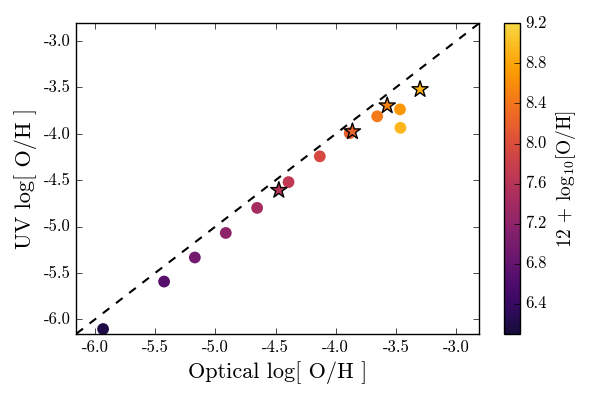
\includegraphics[width=\linewidth]{figs/f1.png}
    \caption{Comparison of direct-method metallicities in the optical direct-method metallicities in the UV. Circular markers show predictions from the Cloudy photoionization code while star markers show predictions from the Mappings photoionization code. Color indicates the input gas-phase oxygen abundance and the black dashed line shows a one-to-one correlation. While the UV direct-temperature calculation systematically predicts lower metallicities than the optical direct-method calculation, the predictions are correlated.}
    \label{fig:UVoptZ}
  \end{center}
\end{figure}
%-------------------------------------------------------

\subsection{Strong-line metallicities}

The \mage galaxies and the other lensed galaxies  have optical metallicities based on strong line methods, which have been converted to the ``standard'' \citet{Pettini+2004} (hereafter PP04) N2O2 abundance scale using the empirical calibration from \citet{Kewley+2008}. We compute N2O2 strong line abundances for our model grid using the equation from PP04:

\begin{equation}
12 + \logOH = 8.90 + 0.57 \times \log_{10}(\mathrm{[N\,II]}/\mathrm{H}\alpha)
\end{equation}


\subsection{Theoretical metallicity calibration}\label{sec:model:corr}

There is a known offset between absolute abundances (i.e., the true specified gas phase abundances in the photoionization models) and the abundances calculated from strong line and direct-temperature methods (i.e., the gas phase abundances one would infer from the models based on emission line strengths) in photoionization models \citep{Kewley+2008}. We must correct for this offset before we can compare our photoionization model metallicities with observations on the same scale. The correction is small at low metallicities (\logOH$ \lesssim 8$), $\lesssim 0.1$\,dex. At metallicities above solar metallicity (\logOH$\gtrsim 8.7$) the correction is between 0.2-1.0\,dex, depending on ionization parameter, where models with higher ionization parameters require larger corrections.

\paragraph{Direct-\Te theoretical calibration} At each age, metallicity, and ionization parameter point in the \CloudyFSPS model grid, we calculate an optical direct-method abundance (as described in \S\ref{sec:model:Te}) to determine the offset between the true oxygen abundance in the \Cloudy model and the measured oxygen abundance. We fit a third-order polynomial to the direct temperature oxygen abundance as a function of the true \Cloudy oxygen abundance at each model age and ionization parameter.

\paragraph{Strong line theoretical calibration} We also determine the offset between the true oxygen abundance in the \Cloudy model and the measured strong-line abundance. Following \citet{Kewley+2008}, we use the \citet{Pettini+2004} (hereafter PP04) N2 metallicity as the ``standard'' abundance indicator. At each age, metallicity, and ionization parameter point in the \CloudyFSPS model grid, we calculate PP04-N2 abundances. We fit a linear function to the strong line abundance as a function of true \Cloudy oxygen abundance at each model age and ionization parameter.

We show the resultant theoretical abundance calibration for constant SFR models at 10\Myr in Fig.~\ref{fig:offset}. The $x$-axis shows the ``true'' oxygen abundance, as specified in \Cloudy, and the $y$-axis shows the abundance calculated from the direct-\Te method (left) and the PP04-N2 method (right). In both panels, the blue lines show the fit used for the theoretical correction, color-coded by ionization parameter. The fitted line is a third-order polynomial for direct-\Te abundances (left) and a linear function for the strong line abundances (right). These fits are provided in the Appendix.

%-------------------------------------------------------
% Figure 2:
%-------------------------------------------------------
\begin{figure*}
  \begin{center}
    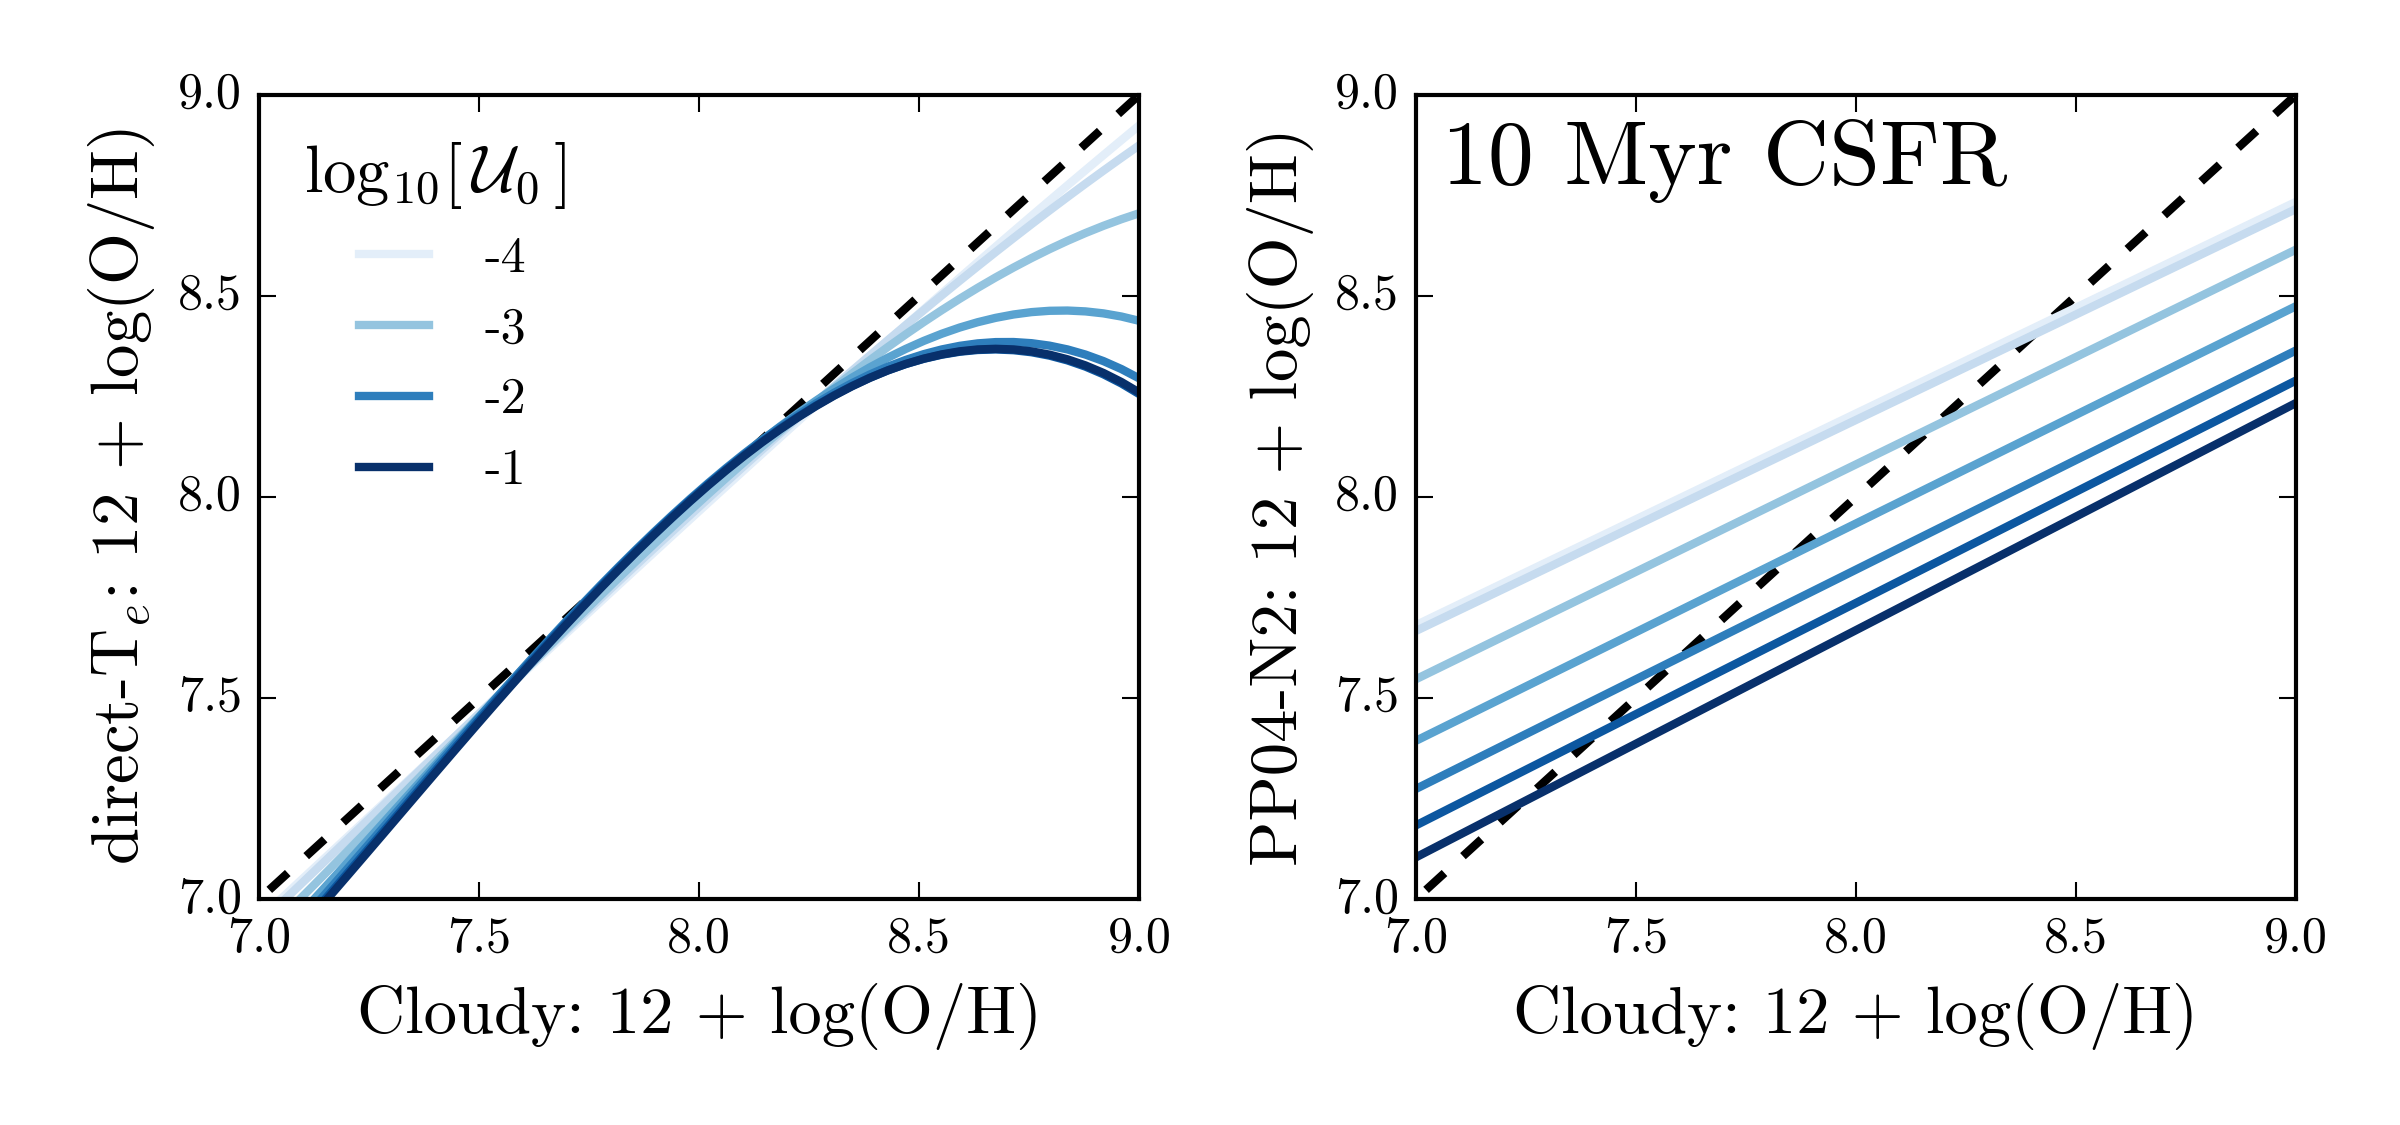
\includegraphics[width=\linewidth]{figs/f2.png}
    \caption{Metallicity offsets for the direct-\Te method (left) and the PP04-N2 method (right). The $x$-axis shows the absolute oxygen abundance input to \Cloudy. The $y$-axis shows the metallicity derived from emission line strengths using the respective metallicity calculations. Each line represents the polynomial fit to the models at each ionization parameter used in the model. The lines are color-coded by ionization parameter, from \logUeq{-4} in light blue to \logUeq{-1} in dark blue. The black dashed line shows a one-to-one relationship.}
    \label{fig:offset}
  \end{center}
\end{figure*}
%-------------------------------------------------------

\subsection{Deriving abundances from UV diagnostic diagrams}\label{sec:Z:UV}
We use various combinations of predicted emission line ratios to construct diagnostic diagrams. At a given model age, variations in ionization parameter and gas phase abundances change the emission line ratios, producing a surface in the diagnostic diagram. Then, for each galaxy, we can compare the observed emission line ratios to the model emission line ratios to to infer the gas phase abundance. Specifically, the emission line ratios ($x$, $y$) for a given galaxy are matched to the surface of the model grid by smoothly interpolating between points in ionization parameter and metallicity.

This approach can be sensitive to slight shifts in the observed emission line ratios, so we use a Monte-Carlo method to estimate errors on this UV-derived metallicity. For each object, we draw $N=1000$ samples from a gaussian distribution centered at the observed $x$,$y$ coordinate  with width equal to the reported emission line ratio errors. We re-measure the metallicity at each of these 1000 samples, using the median of the resultant metallicity distribution as the final UV-derived metallicity. The 16$^{th}$ and 84$^{th}$ percentiles of the metallicity distribution then provide the upper and lower error limits, respectively.

This metallicity corresponds to the absolute gas phase abundance from \Cloudy. However, if we want to compare the UV-derived metallicity with the metallicity derived from optical emission lines, we need to rescale the \Cloudy metallicity according to our theoretical abundance calibrations from \S\ref{sec:model:corr}. For the \citet{Berg+2016} galaxies  with optical direct-\Te metallicities, we apply the direct-\Te correction described in \S\ref{sec:model:corr}. For the \mage galaxies with optical strong line metallicities, we apply the relevant strong line correction described in \S\ref{sec:model:corr}. In general, the metallicity correction changes the UV-derived abundance by $<0.1$\,dex at $12 + \logOH < 8$, and by ${\sim}0.1$\,dex at $8.0 < 12 + \logOH < 8.5$.


%%%%%%%%%%%%%%%%%%%%%%%%%%%%%%%%%%%%%%%%%%%%%%%%%%%%%%%%%%%%%%%%%%%%%%%%%%%%%%%%
\section{Abundance comparisons}\label{sec:UVOpt}

\subsection{UV-Optical abundance comparisons}

In this section we compare the metallicities derived from UV diagnostic diagrams (\S\ref{sec:Z:UV}) with metallicities derived using optical emission lines and evaluate the utility of the UV diagnostic diagrams as metallicity indicators.

\subsubsection{Diagnostics using \ciii$\lambda$1906,1909}\label{sec:UVOpt:C}

\ciii$\lambda$1906,1909 are the brightest emission lines after Ly-$\alpha$ in the UV spectra of star-forming galaxies, which makes the lines desirable candidates to use in emission line diagnostics. Several analyses of UV emission line spectra have suggested diagnostics using \ciii$\lambda$1906,1909, including \citet{Feltre+2016, Jaskot+2016, Byler+2018}. In \citet{Byler+2018}, we highlighted the potential of the Si3C3 \vs O3C3 diagnostic diagram, which uses the \SiuIII$\lambda$1883, \ciii$\lambda$1906, and \oiii$\lambda$1666 emission lines. These emission lines are relatively bright and easy to detect, and are closely spaced in wavelength to minimize dust extinction errors.

In the left panel of Fig.~\ref{fig:UVC} we show the Si3C3-O3C3 diagnostic diagram as presented in \citet{Byler+2018}. We compare the model grid with the local BCDs from \citet{Berg+2016} (gold circles), and the high redshift \mage galaxies from \citet{Rigby+2018b} (diamonds). As noted in \citet{Byler+2018}, the model grid is able to reproduce the observed range of line ratios in samples of both low and high-redshift galaxies.

We use the Si3C3-O3C3 diagnostic grid to derive UV metallicities, which we compare to the optical metallicities in the right panel of Fig.~\ref{fig:UVC}. The optically-derived direct-\Te metallicity from \citet{Berg+2016} is shown on the $x$-axis, and the UV metallicity derived using the Si3C3-O3C3 is shown on the $y$-axis. For the \mage galaxies, the $x$-axis shows the optical metallicity from O3N3 or $R_{23}$.

The UV and optical metallicities agree within error for ${\sim}80\%$ of the \citet{Berg+2016} galaxies. While the UV-predicted metallicities are largely consistent with the optical, the range in UV metallicities is much larger than the range in optical metallicities. Additionally, there are several objects where the UV metallicity catastrophically fails to match the optical metallicity. These failures do not seem to have an overall bias toward higher or lower metallicities.

%-------------------------------------------------------
% Figure 3:
%-------------------------------------------------------
\begin{figure*}
  \begin{center}
    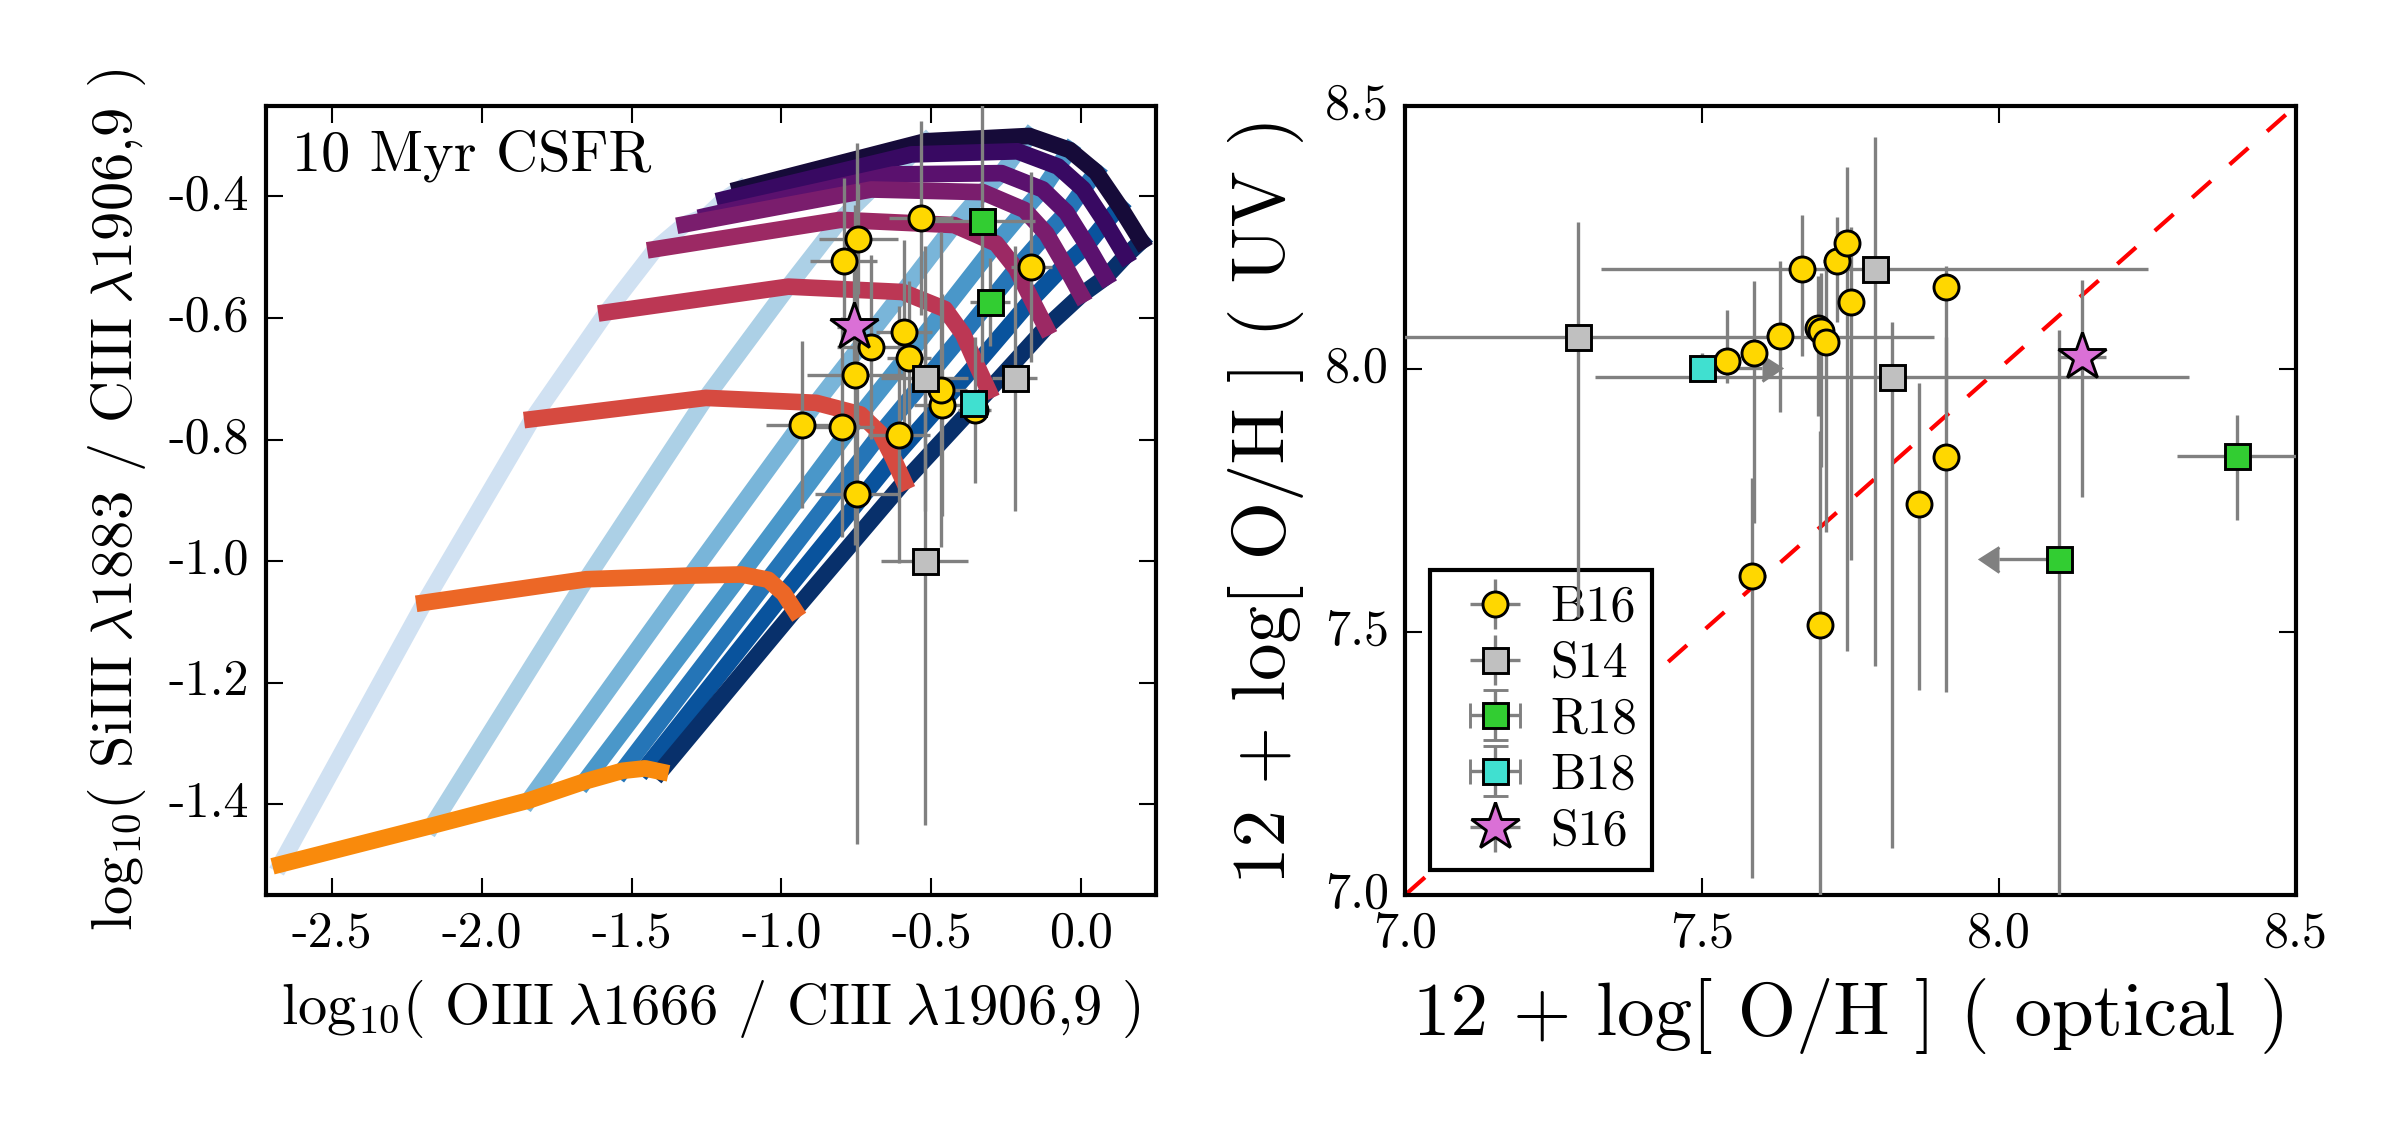
\includegraphics[width=\linewidth]{figs/f3.png}
    \caption{\emph{Left:} UV diagnostic diagram presented in \citet{Byler+2018}, comparing emission line ratio \oiii$\lambda$1666 / \ciii$\lambda$1906 with \SiuIII$\lambda$1883 / \ciii$\lambda$1906. The blue lines connect models of constant ionization parameter, from \logUeq{-1} (dark blue) to \logUeq{-4} (light blue). Models of constant metallicity are shown from \logZeq{-2} (purple) to \logZeq{0} (orange). \emph{Right:} Metallicity derived using the Si3C3 / O3C3 UV diagnostic (right) compared to the optical metallicity. The dashed line shows a one-to-one relationship. In both panels, the gold circles are the sample of local BCDs from \citet{Berg+2016}. The grey squares are high-redshift galaxies from \citet{Stark+2014}, the green diamonds are high-redshift galaxies from \citet{Rigby+2018b}, and the turquoise square is a high-redshift galaxy from \citet{Berg+2018}. The pink star is the stacked spectrum of high-redshift galaxies from \citet{Steidel+2016}.}
    \label{fig:UVC}
  \end{center}
\end{figure*}
%-------------------------------------------------------

\subsubsection{Diagnostics using \heii$\lambda$1640}\label{sec:UVOpt:He}

\heii$\lambda$1640 emission has been detected in both local and high-redshift galaxies and is one of the brighter UV emission lines, making it another desirable line to use in a metallicity diagnostic. The \heii$\lambda$1640 line has been used in several proposed emission line diagnostics \citep[e.g.,][]{Jaskot+2016, Feltre+2016}, including the He2C3-O3C3 diagnostic presented in \citet{Byler+2018}, which uses the \heii$\lambda$1640, \ciii$\lambda$1906, and \oiii$\lambda$1666 emission lines. In \citet{Byler+2018}, however, we did note that observations of \heii$\lambda$1640 emission can include contributions from both nebular emission and stellar wind emission, making it a potentially problematic metallicity tracer.

In the left panel of Fig.~\ref{fig:UVHe} we show the He2C3-O3C3 diagram and show that the model grid is able to reproduce the range of observed emission line ratios. The right panel of Fig.~\ref{fig:UVHe} compares the UV metallicities with the optical metallicities. Fig.~\ref{fig:UVHe} shows that the UV and optical metallicities are in most of the comparison sample. In general, the disagreement between the UV and optical metallicities is much smaller than in Fig.~\ref{fig:UVC}, with consistent UV and optical metallicities in most of the observed galaxies. However, the UV metallicities are biased to systematically lower metallicities in the \mage galaxies (green diamonds) by as much as 1\,dex in the \mage galaxies, with little correlation with optical metallicity.

Broad \heii emission in galaxies is commonly interpreted as an indication of the presence of W-R stars \citep[e.g., ][]{Kunth+1985,Conti+1991, Schaerer+1999, Brinchmann+2008}. W-R stars are more common in metal-rich stellar populations ($12+\logOH \gtrsim 8$), with the strongest \heii emission associated with populations at solar metallicity or higher. Most of the objects in the \citet{Berg+2016} BCD sample have low enough metallicities that the contribution from stellar emission should be small (${\sim}$25\% of the nebular emission flux), however, broad \heii$4686\ang$ emission is detected in a handful of objects. We expect that any contamination from stellar \heii emission would be worse in the \mage galaxies, because these galaxies have metallicities near solar or higher.

We discuss the issues associated with diagnostics that use \civ, \ciii, or \heii emission lines at length in \S\ref{sec:discussion}.

%-------------------------------------------------------
% Figure 4:
%-------------------------------------------------------
\begin{figure*}
  \begin{center}
    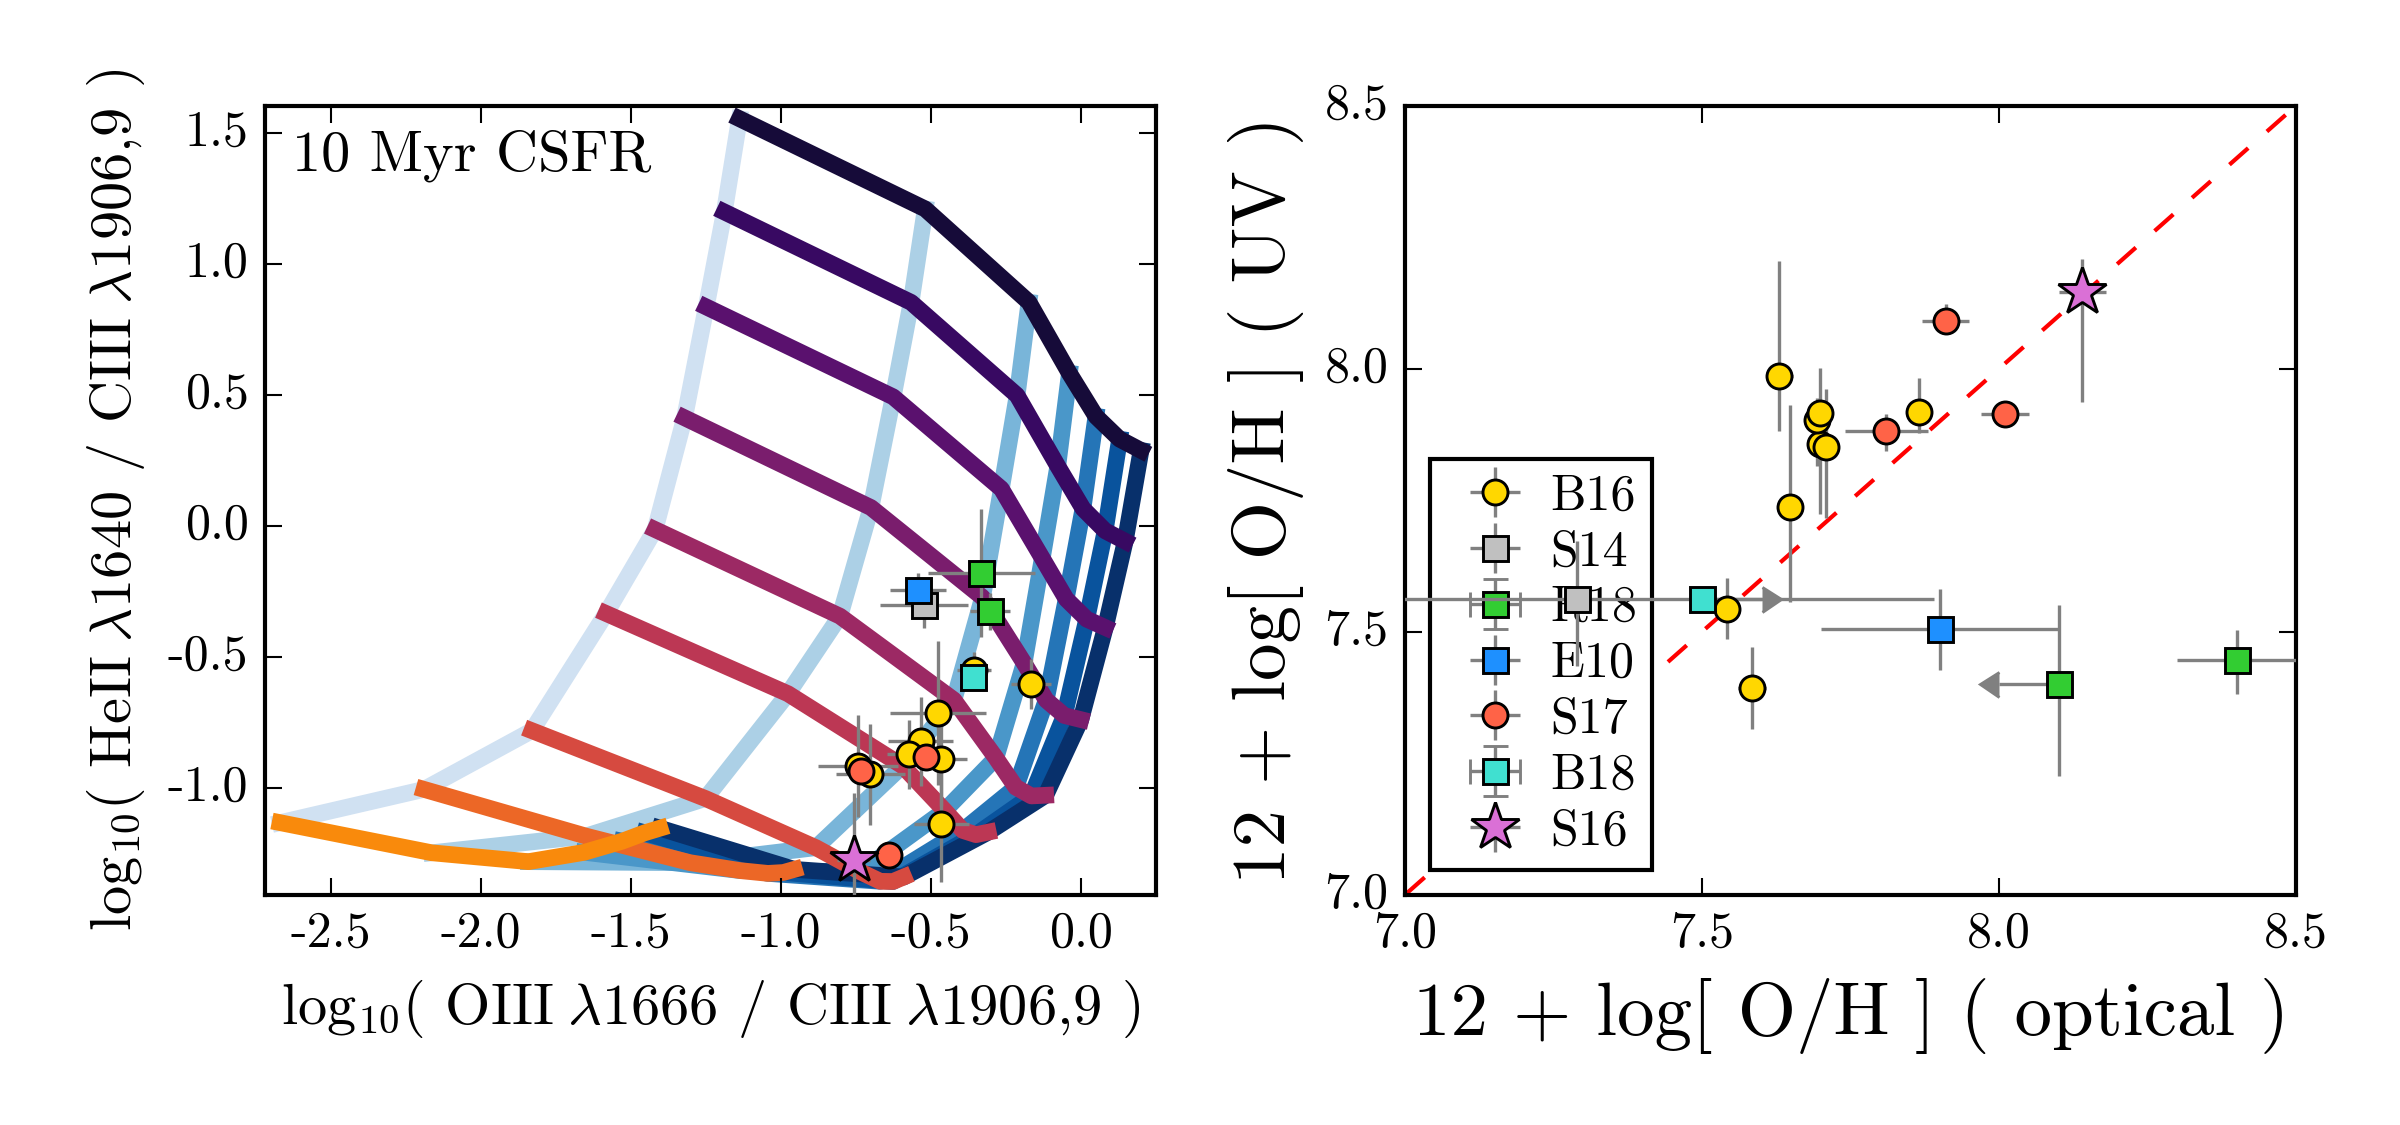
\includegraphics[width=\linewidth]{figs/f4.png}
    \caption{\emph{Left:} The He2C3 / O3C3 diagnostic diagram.  The blue lines connect models of constant ionization parameter, from \logUeq{-1} (dark blue) to \logUeq{-4} (light blue). Models of constant metallicity are shown from \logZeq{-2} (purple) to \logZeq{0} (orange). The gold and red circles are the sample of local BCDs from \citet{Berg+2016} and \citet{Senchyna+2017}, respectively. The grey squares show high-redshift galaxies from \citet{Stark+2014} and the green squares show the high-redshift galaxies from \citet{Rigby+2018b}. The blue square is the high redshift galaxy from \citet{Erb+2010}, and the cyan square is the high redshift galaxy from \citet{Berg+2018}. \emph{Right:} Metallicities predicted by the He3C3 / O3C3 diagnostic compared to optically-derived metallicities. The dashed line shows a one-to-one relationship. The UV and optical metallicities are correlated for most of the galaxies, particularly the metal-poor local BCD galaxies. For the comparitively metal-rich \mage galaxies, the UV diagnostic significantly underpredicts optical metallicities.}
    \label{fig:UVHe}
  \end{center}
\end{figure*}
%-------------------------------------------------------

\subsubsection{Diagnostics using \civ$\lambda$1548,1550}\label{sec:UVOpt:CIV}

We show the \civ$1548,1550$\ang / \oiii$1666$\ang \vs \oiii$1666$\ang / \ciii$1906,1908$\ang (C4O3 - O3C3) diagnostic diagram in the left panel of Fig.~\ref{fig:UVCIV}. Most of the galaxies from the observational comparison sample have larger C4O3 ratios than predicted by the models. At the metallicities associated with the local BCD sample ($12+\logOH \sim 7.5-8$), the stellar+nebular \civ emission models from \citet{Byler+2018} predict that stellar contamination can change the C4O3 ratio by 0.1-0.3\,dex. Contamination from stellar emission is less of an issue for the galaxies from \citet{Senchyna+2017} (red points), since the higher spectral resolution of the observations allowed the authors to fit for both the broad and narrow \civ emission components.
We show the comparison between UV and optical metallicities for the C4O3-O3C3 diagnostic in the right panel of Fig.~\ref{fig:UVCIV}. Unsurprisingly, the mismatch between observed and model line ratios in the left panel of Fig.~\ref{fig:UVCIV} translates to poor agreement between the UV and optical metallicities in the right panel. For all objects, the UV metallicity is larger than the optical metallicity, by 0.1 to 0.7\,dex, and an average offset of 0.3\,dex. Only three objects have UV metallicities consistent with their optical estimates within the errors. There is some evidence for a metallicity-dependent offset, where the metal-rich objects show somewhat more scatter. The \citet{Senchyna+2017} galaxies show the smallest offset, potentially due to the fact that the C4 emission line fluxes are ``nebular only''. More generally, the C4O3-O3C3 emission line ratios seem to be a poor metallicity diagnostic.

We note the absence of the \mage galaxies in Fig.~\ref{fig:UVCIV}. Inspection of the \civ emission feature in these comparatively metal-rich objects revealed strong stellar emission with the signature P-Cygni profile, with little or no evidence for nebular emission.

%-------------------------------------------------------
% Figure 5:
%-------------------------------------------------------
\begin{figure*}
  \begin{center}
    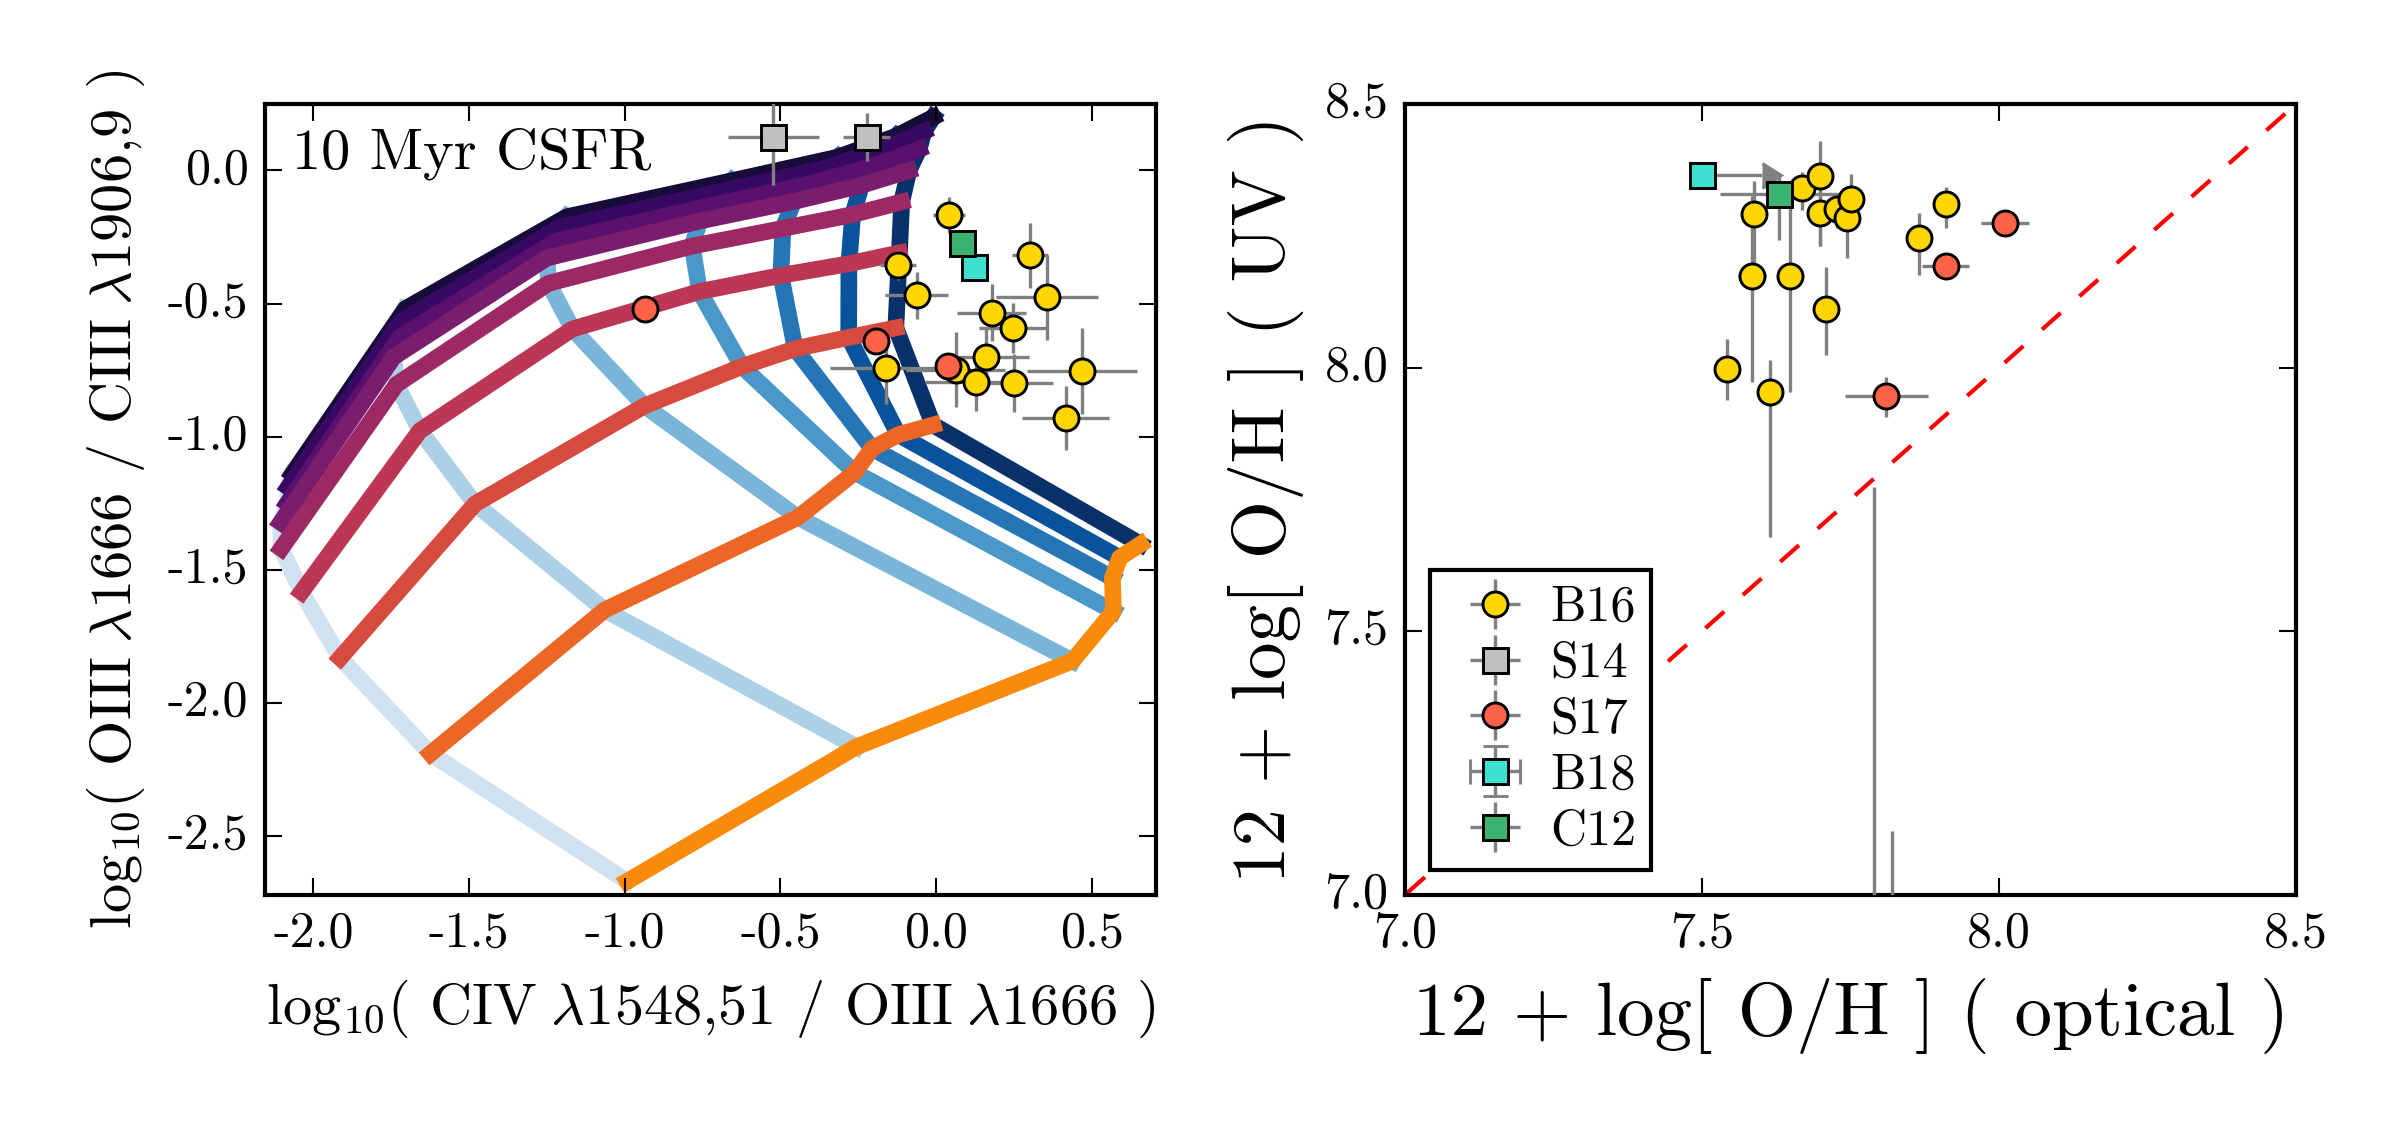
\includegraphics[width=\linewidth]{figs/af4.png}
    \caption{\emph{Left:} The C4O3 / O3C3 diagnostic diagram. The blue lines connect models of constant ionization parameter, from \logUeq{-1} (dark blue) to \logUeq{-4} (light blue). Models of constant metallicity are shown from \logZeq{-2} (purple) to \logZeq{0} (orange). The gold and red circles are the sample of local BCDs from \citet{Berg+2016} and \citet{Senchyna+2017}, respectively. The grey squares show high-redshift galaxies from \citet{Stark+2014} and the green squares show the high-redshift galaxies from \citet{Rigby+2018b}. The blue square is the high redshift galaxy from \citet{Christensen+2012}, and the cyan square is the high redshift galaxy from \citet{Berg+2018}. Many of the galaxies have CIVO3 ratios that are larger than predicted by the models, in many cases due to contamination from stellar wind emission in the \civ emission line. Harder ionizing spectra could also help explain the offset. \emph{Right:} Metallicities predicted by the C4O3 / O3C3 diagnostic compared to optically-derived metallicities. The dashed line shows a one-to-one relationship. The UV diagnostic predicts metallicities that are 0.3-0.5 dex larger than the optical metallicities.}
    \label{fig:UVCIV}
  \end{center}
\end{figure*}
%-------------------------------------------------------

\subsubsection{Diagnostics using silicon and oxygen lines}\label{sec:UVOpt:SiO}

There are plenty of emission line diagnostics that do not include \civ, \ciii, or \heii lines that may provide a more robust estimate of the gas phase metallicity. Unfortunately, the \citet{Berg+2016} sample only includes emission line measurements for \civ, \heii, \oiii, \SiuIII, and \ciii, which means that this sample cannot be used to calibrate any of the non-carbon, non-helium UV diagnostics. For these diagnostics, we must rely on the \mage sample for UV-optical comparisons.

UV-optical comparisons using the \mage sample will differ in two important ways. First, only seven of the 13 \mage galaxies studied here have optical metallicity measurements, and only two of these seven have four or more non-carbon, non-helium emission line detections, to compare with diagnostic diagrams. Second, the optical metallicities from the \mage sample are from empirically calibrated strong-line methods like $R_{23}$ or O3N2, rather than the more robust direct-\Te method metallicities from the \citet{Berg+2016} sample. Nonetheless, these galaxies provide a crucial link between UV and optical abundance determinations, and even upper limits can provide a useful quantitative calibration.

In this work we analyze 12 UV diagnostic diagrams that do not include carbon lines or \heii$\lambda$1640, listed in Table~\XXX. We chose these diagnostics such that the combination of emission lines used provided the maximum possible overlap with the \mage galaxy observations.

In Fig.~\ref{fig:UVSiO} we highlight four of these diagnostic diagrams. The diagnostics in Fig.~\ref{fig:UVSiO} have the same line ratio on the $x$-axis, \SiuII$\lambda$1307 / \SiuII$\lambda$1531 (Si2Si2), and on the $y$-axis we show \SiuIII$\lambda$1883 / \oii$\lambda$2471  (Si3O2; top left), \SiuIII$\lambda$1883 / \nii$\lambda$2142 (Si3N2; top right), \oii$\lambda$2471 / \oiii$\lambda$1666 (O2O3; bottom left), and \niii$\lambda$1750 / \nii$\lambda$2142 (N3N2; bottom right). Each diagnostic in Fig.~\ref{fig:UVSiO} is compared with \mage galaxy observations from \citet{Rigby+2018b} (coloured diamonds) for objects where all four emission lines were detected. In all diagrams, the model grids are able to reproduce the observed range in emission line ratios, within error.

The \mage galaxies have higher metallicities than the \citet{Berg+2016} sample of galaxies (\logOH${\sim}8.5$, compared to \logOH${\sim}7.5$), and in general, the \mage galaxies in Fig.~\ref{fig:UVSiO} do occupy regions of the model grid associated with higher metallicities. Additionally, galaxies that appear in multiple panels of Fig.~\ref{fig:UVSiO} are generally found in consistent regions of the \logU$-$\logZ model grid.





Our evaluation of the diagnostics from Table~\XXX will proceed along two paths. First, using the larger sample of \mage galaxies, we will determine if metallicities derived using different UV diagnostics are consistent with one another. Second, we will compare the UV and optical metallicities for RCS0327 and S1527, the two \mage galaxies with both UV and optical metallicities.

%-------------------------------------------------------
% Figure 5:
%-------------------------------------------------------
\begin{figure*}
  \begin{center}
    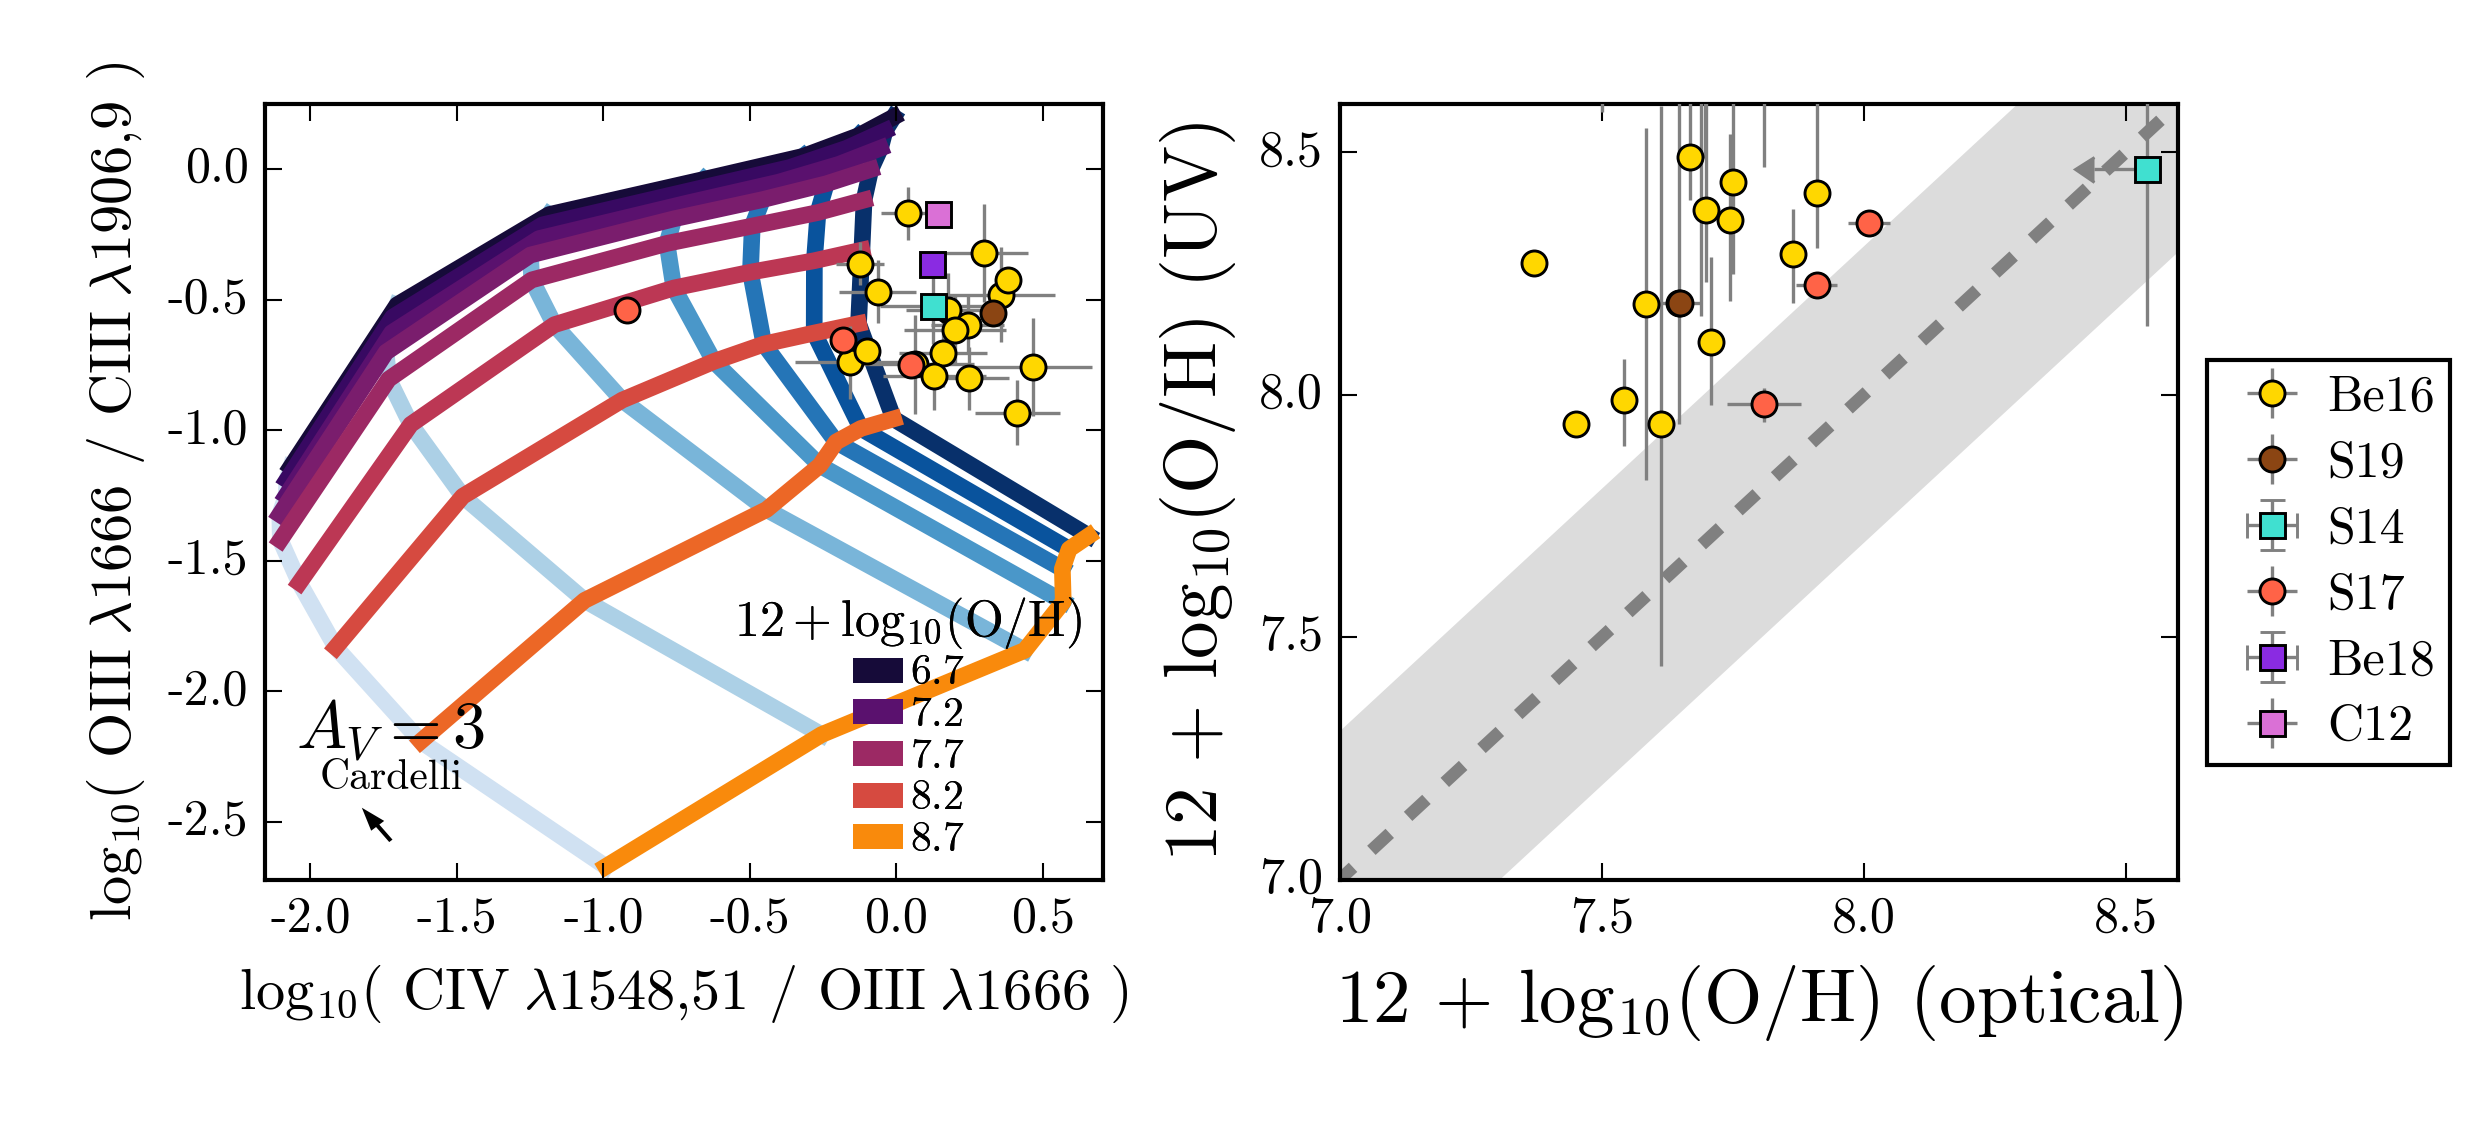
\includegraphics[width=\linewidth]{figs/f5.png}
    \caption{UV diagnostic diagrams using pairs of emission lines excluding carbon species and \heii$\lambda$1640.  The blue lines connect models of constant ionization parameter, from \logUeq{-1} (dark blue) to \logUeq{-4} (light blue). Models of constant metallicity are shown from \logZeq{-2} (purple) to \logZeq{0} (orange). The colored diamonds show the high-redshift galaxies from \citet{Rigby+2018b}. There are few galaxies where all four emission lines used in a given diagnostic diagram are observed in multiple objects. For galaxies that appear in multiple diagrams, the position in ionization parameter - metallicity space is roughly consistent between diagnostics.}
    \label{fig:UVSiO}
  \end{center}
\end{figure*}
%-------------------------------------------------------

In Fig.~\ref{fig:UVZ} we compare the optical metallicity of RCS0327 and S1527 to various UV metallicities, as derived using different diagnostics. The optical metallicity is shown on the $x$-axis, while the UV metallicity is shown on the $y$-axis. The marker color indicates the specific UV diagnostic used, labeled on the color bar. While RCS0327 has a single optical metallicity measurement, the rest-UV spectroscopy targets multiple spatial locations corresponding to several distinct star-forming knots. We separate the knots (E,G, U) on the $x$-axis of Fig.~\ref{fig:UVZ} for visual clarity, with an offset of $\pm 0.1$\,dex from the globally averaged optical metallicity, shown at the location of knot-G. The knots are also separated because, in principle, the gas properties could vary significantly between knots. We leave this analysis to a future publication, Byler et al., \emph{in prep}.

We can see from Fig.~\ref{fig:UVZ} that the UV-derived metallicities are consistent with the optical metallicities, within error. The consistency between the UV and optical metallicities in Fig~\ref{fig:UVZ} may indicate that UV diagnostics using silicon and oxygen lines are more robust than those using carbon or helium emission lines.

In general, the various UV metallicities for each object agree with one another, with a scatter of 0.2-0.3\,dex. However, as discussed in \S\ref{sec:UVOpt:UV}, some of the diagnostics provide less reliable metallicity estimates. We found that the Si2Si2-Si2Si3 diagnostic (light blue diamonds in Fig.~\ref{fig:UVZ}) produced metallicities that were systematically higher than other diagnostics. The Si2Si2-Si2Si3 lines were all observable in RCS0327-U and S1527, shown in Fig.~\ref{fig:UVZ}. For RCS0327 the Si2Si2-Si2Si3 metallicity shows the largest offset from the optical metallicity, more than 0.5\,dex. For S1527, the Si2Si2-Si2Si3 diagnostic predicts a metallicity at the upper limit set by the optical \nii/\ha ratio. In both cases, it is reasonable to claim that the Si2Si2-Si2Si3 metallicity is biased to systematically high metallicities.

The best of the diagnostics identified in \S\ref{sec:UVOpt:UV} included Si2Si2-O3Si3 (bright green), Si2O3-Si3O2 (brown), Si2Si2-N3Si3 (pale orange), and Si2Si2-O2O3 (pale red). In Fig.~\ref{fig:UVZ}, these diagnostics show very little scatter in individual objects, (e.g., the pale red and bright green diamonds for knot-G), by design. We also note that these diagnostics provide the closest match to the measured optical metallicity in several objects, which is encouraging.

%-------------------------------------------------------
% Figure 7:
%-------------------------------------------------------
\begin{figure*}
  \begin{center}
    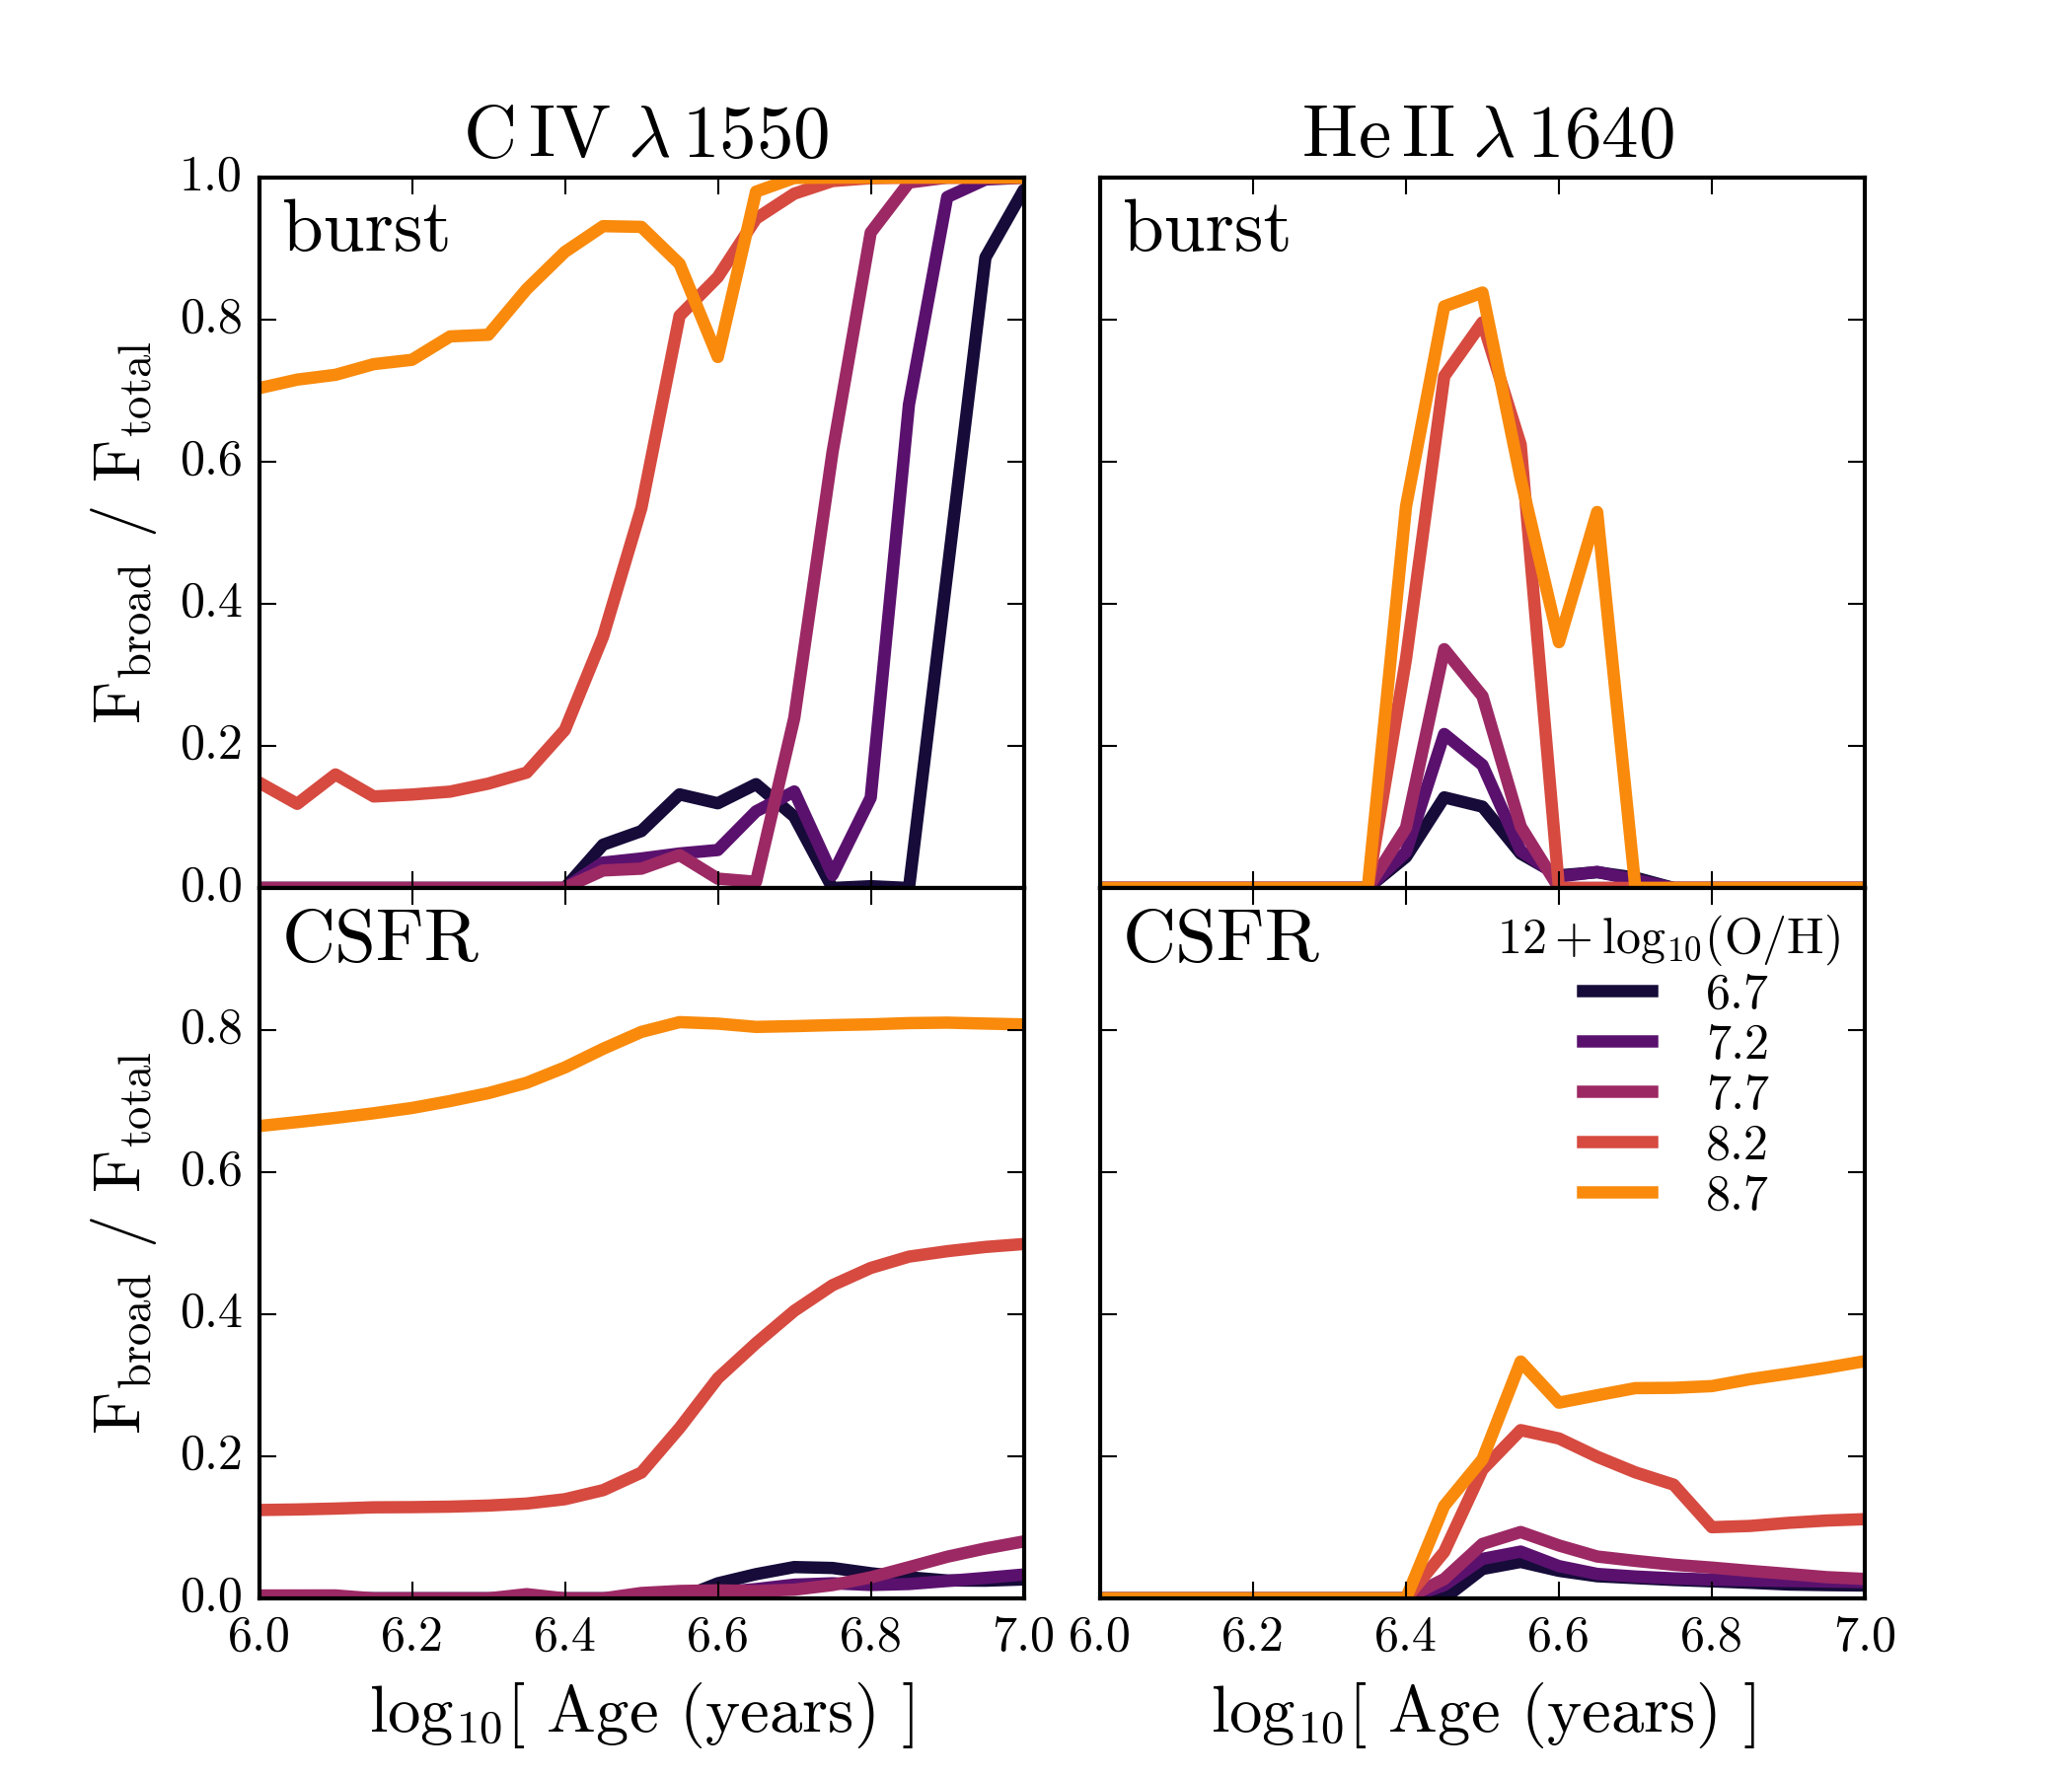
\includegraphics[width=\linewidth]{figs/f7.png}
    \caption{UV metallicities ($y$-axis) derived from various diagnostic diagrams compared to the optical metallicity ($x$-axis). Marker color indicates the different emission line ratios used, and the red dashed line shows a one-to-one relation. RCS0327 has a single optical metallicity measurement spatially averaged over the face of the galaxy, but rest-UV spectra that cover several different spatial locations (e.g., U,G,E,B), which have been shifted on the $x$-axis for visual clarity. The optical metallicity for S1527 only provides an upper limit.}
    \label{fig:UVZ}
  \end{center}
\end{figure*}
%-------------------------------------------------------

\subsection{UV-UV abundance comparisons}\label{sec:UVOpt:UV}

We quantify the robustness of the UV metallicities by looking for consistent predictions between different UV diagnostics. For this consistency check, we use the 12 UV diagnostics identified in Table~\XXX.

Fig.~\ref{fig:UVUV} shows the gas phase oxygen abundance predicted by each of the 12 diagnostics, compared with the oxygen abundance derived using each of the 11 other diagnostics. The rows and columns are labeled with the diagnostic plotted on the $x$- and $y$-axis, respectively. The red dashed line represents unity, and the \mage galaxies are shown with colored diamonds, as indicated in the figure legend.

It is evident from Fig.~\ref{fig:UVUV} that some diagnostics are more consistent than others. For example, the \SiuII$\lambda$1307/\SiuII$\lambda$1531 \vs \SiuII$\lambda$1307/\SiuIII$\lambda$1883 diagnostic (Si2Si2-Si2Si3; first column, $y$-axis) predicts metallicities that are systematically higher than those predicted by other diagnostics by 0.2-0.4\,dex. Encouragingly, though, there are a number of diagnostics that predict metallicities that are well-matched with predictions from other diagnostics. The \SiuII$\lambda$1307/\SiuII$\lambda$1531 \vs \oiii$\lambda$1666/\SiuIII$\lambda$1883 diagnostic (Si2Si2-O3Si3; third row, $x$-axis, and fourth column, $y$-axis) is quite promising, because these emission lines are observed in a number of galaxies and the predicted metallicities agree with several other diagnostics.

In general, the diagnostics using a single species (e.g., all silicon lines) have the least consistent metallicity predictions. Diagnostics that include a mix of ionization states (e.g. \oiii and \oii) seem to produce more consistent metallicity predictions. From Fig.~\ref{fig:UVUV}, other promising diagnostics include:
\begin{itemize}
    \item \SiuII$\lambda$1307/\oiii$\lambda$1666 \vs \SiuIII$\lambda$1883/\oii$\lambda$2471 (Si2O3-Si3O2; 11th row, $x$-axis and 12th column, $y$-axis)
    \item \SiuII$\lambda$1307/\SiuII$\lambda$1531 \vs \niii1750/\SiuIII1883 (Si2Si2-N3Si3; 6th row $x$-axis, 7th column $y$-axis)
    \item \SiuII$\lambda$1307/\SiuII$\lambda$1531 \vs \oii$\lambda$2471/\oiii$\lambda$1666 (Si2Si2-O2O3; 4th row $x$-axis, 5th column $y$-axis)
\end{itemize}

Only one galaxy has observed \mgii$\lambda$2796 emission. The diagnostic that includes \mgii$\lambda$2796 also produces systematically low metallicity estimates. However, the \mgii$\lambda$2796 emission may not have a nebular origin; \citet{Rigby+2018a} suggests the \mgii$\lambda$2796 emission is the result of continuum upscattering.

%-------------------------------------------------------
% Figure 6:
%-------------------------------------------------------
\begin{figure*}
  \begin{center}
    \includegraphics[width=\linewidth]{figs/f6.png}
    \caption{Consistency between UV-derived metallicities. We show the gas phase oxygen abundance ($12+$\logOH) measured with twelve different UV-diagnostics, as labeled on the outer edges of the figure. The diagnostic labeled on each row is plotted on the $x$-axis, while the diagnostic labeled on the columns is plotted on the $y-$axis. \mage galaxies are shown with colored diamonds and the red dashed line shows a one-to-one relationship. The \SiuII$\lambda$1307/\SiuII$\lambda$1531 \vs \oiii$\lambda$1666/\SiuIII$\lambda$1883 diagnostic (the third row, $x$-axis and the fourth column, $y$-axis) predicts metallicities that are consistent with most other diagnostics. In contrast, the \SiuII$\lambda$1307/\SiuII$\lambda$1531 \vs \SiuII$\lambda$1307/\SiuIII$\lambda$1883 diagnostic (first column, $y$-axis) predicts metallicities that are systematically higher than other diagnostics.}
    \label{fig:UVUV}
  \end{center}
\end{figure*}
%-------------------------------------------------------

\section{UV-derived metallicities}\label{sec:UVZ}

In this section, we derive metallicities for the \mage galaxies using the most promising set of diagnostics from \S\ref{sec:UVOpt}. The \mage galaxies with both UV and optical metallicities can be used to connect studies where only optical or only UV metallicities are available. We first derive metallicities using all 12 diagnostics used in this work. We then propose a new weighting scheme based on the post promising subset of diagnostics identified in \S\ref{sec:UVOpt}, and then calculate UV metallicities for the \mage sample.

Fig.~\ref{fig:UVmage} shows the gas phase oxygen abundance derived using all 12 UV diagnostics for each of the \mage galaxies. Each point is color-coded by the diagnostic used to derive the abundance, using the same scheme as Fig.~\ref{fig:UVZ}, as indicated in the color bar. The diagnostics predict oxygen abundances between $7.75< 12+$\logOH$<8.75$. The spread in predicted metallicities for a given object varies between 0.25 dex and 0.75 dex.

As expected, in Fig.~\ref{fig:UVmage}, the Si2Si2-Si2Si3 diagnostic (pale blue diamonds) predicts the largest oxygen abundances in every object, offset from other predictions by at least $\sim0.25$ dex, and in an extreme case, by as much as 1\,dex. The metallicities predicted with this diagnostic exceed solar metallicity in most cases, which corresponds to gas enrichment that may be difficult to attain at the metallicities in this sample.

The best of the diagnostics identified in \S\ref{sec:UVOpt:UV} included Si2Si2-O3Si3 (bright green diamonds), Si2O3-Si3O2 (brown), Si2Si2-N3Si3 (pale orange), and Si2Si2-O2O3 (pale red). When simultaneously measured in a single object, the spread in predicted metallicity is small, as expected.

From our analysis in \S\ref{sec:UVOpt}, Si2Si2-O3Si3, Si2O3-Si3O2, Si2Si2-N3Si3, and Si2Si2-O2O3 produce the most accurate and precise metallicity estimates. To calculate a final UV metallicity for the galaxies in the \mage sample, we thus propose a weighted average of the metallicities derived with these four diagnostics, following the form \XXX; these metallicities are given in Table.\XXX.

Fig.~\ref{fig:UVmage} shows the "final" UV metallicity calculated for each of the \mage galaxies, now plotted as a function of redshift. For comparison, we also compare the metallicities and redshifts from blah (\XXX actually make this plot; not sure if this is the best way to summarize results).

%-------------------------------------------------------
% Figure 8:
%-------------------------------------------------------
\begin{figure*}
  \begin{center}
    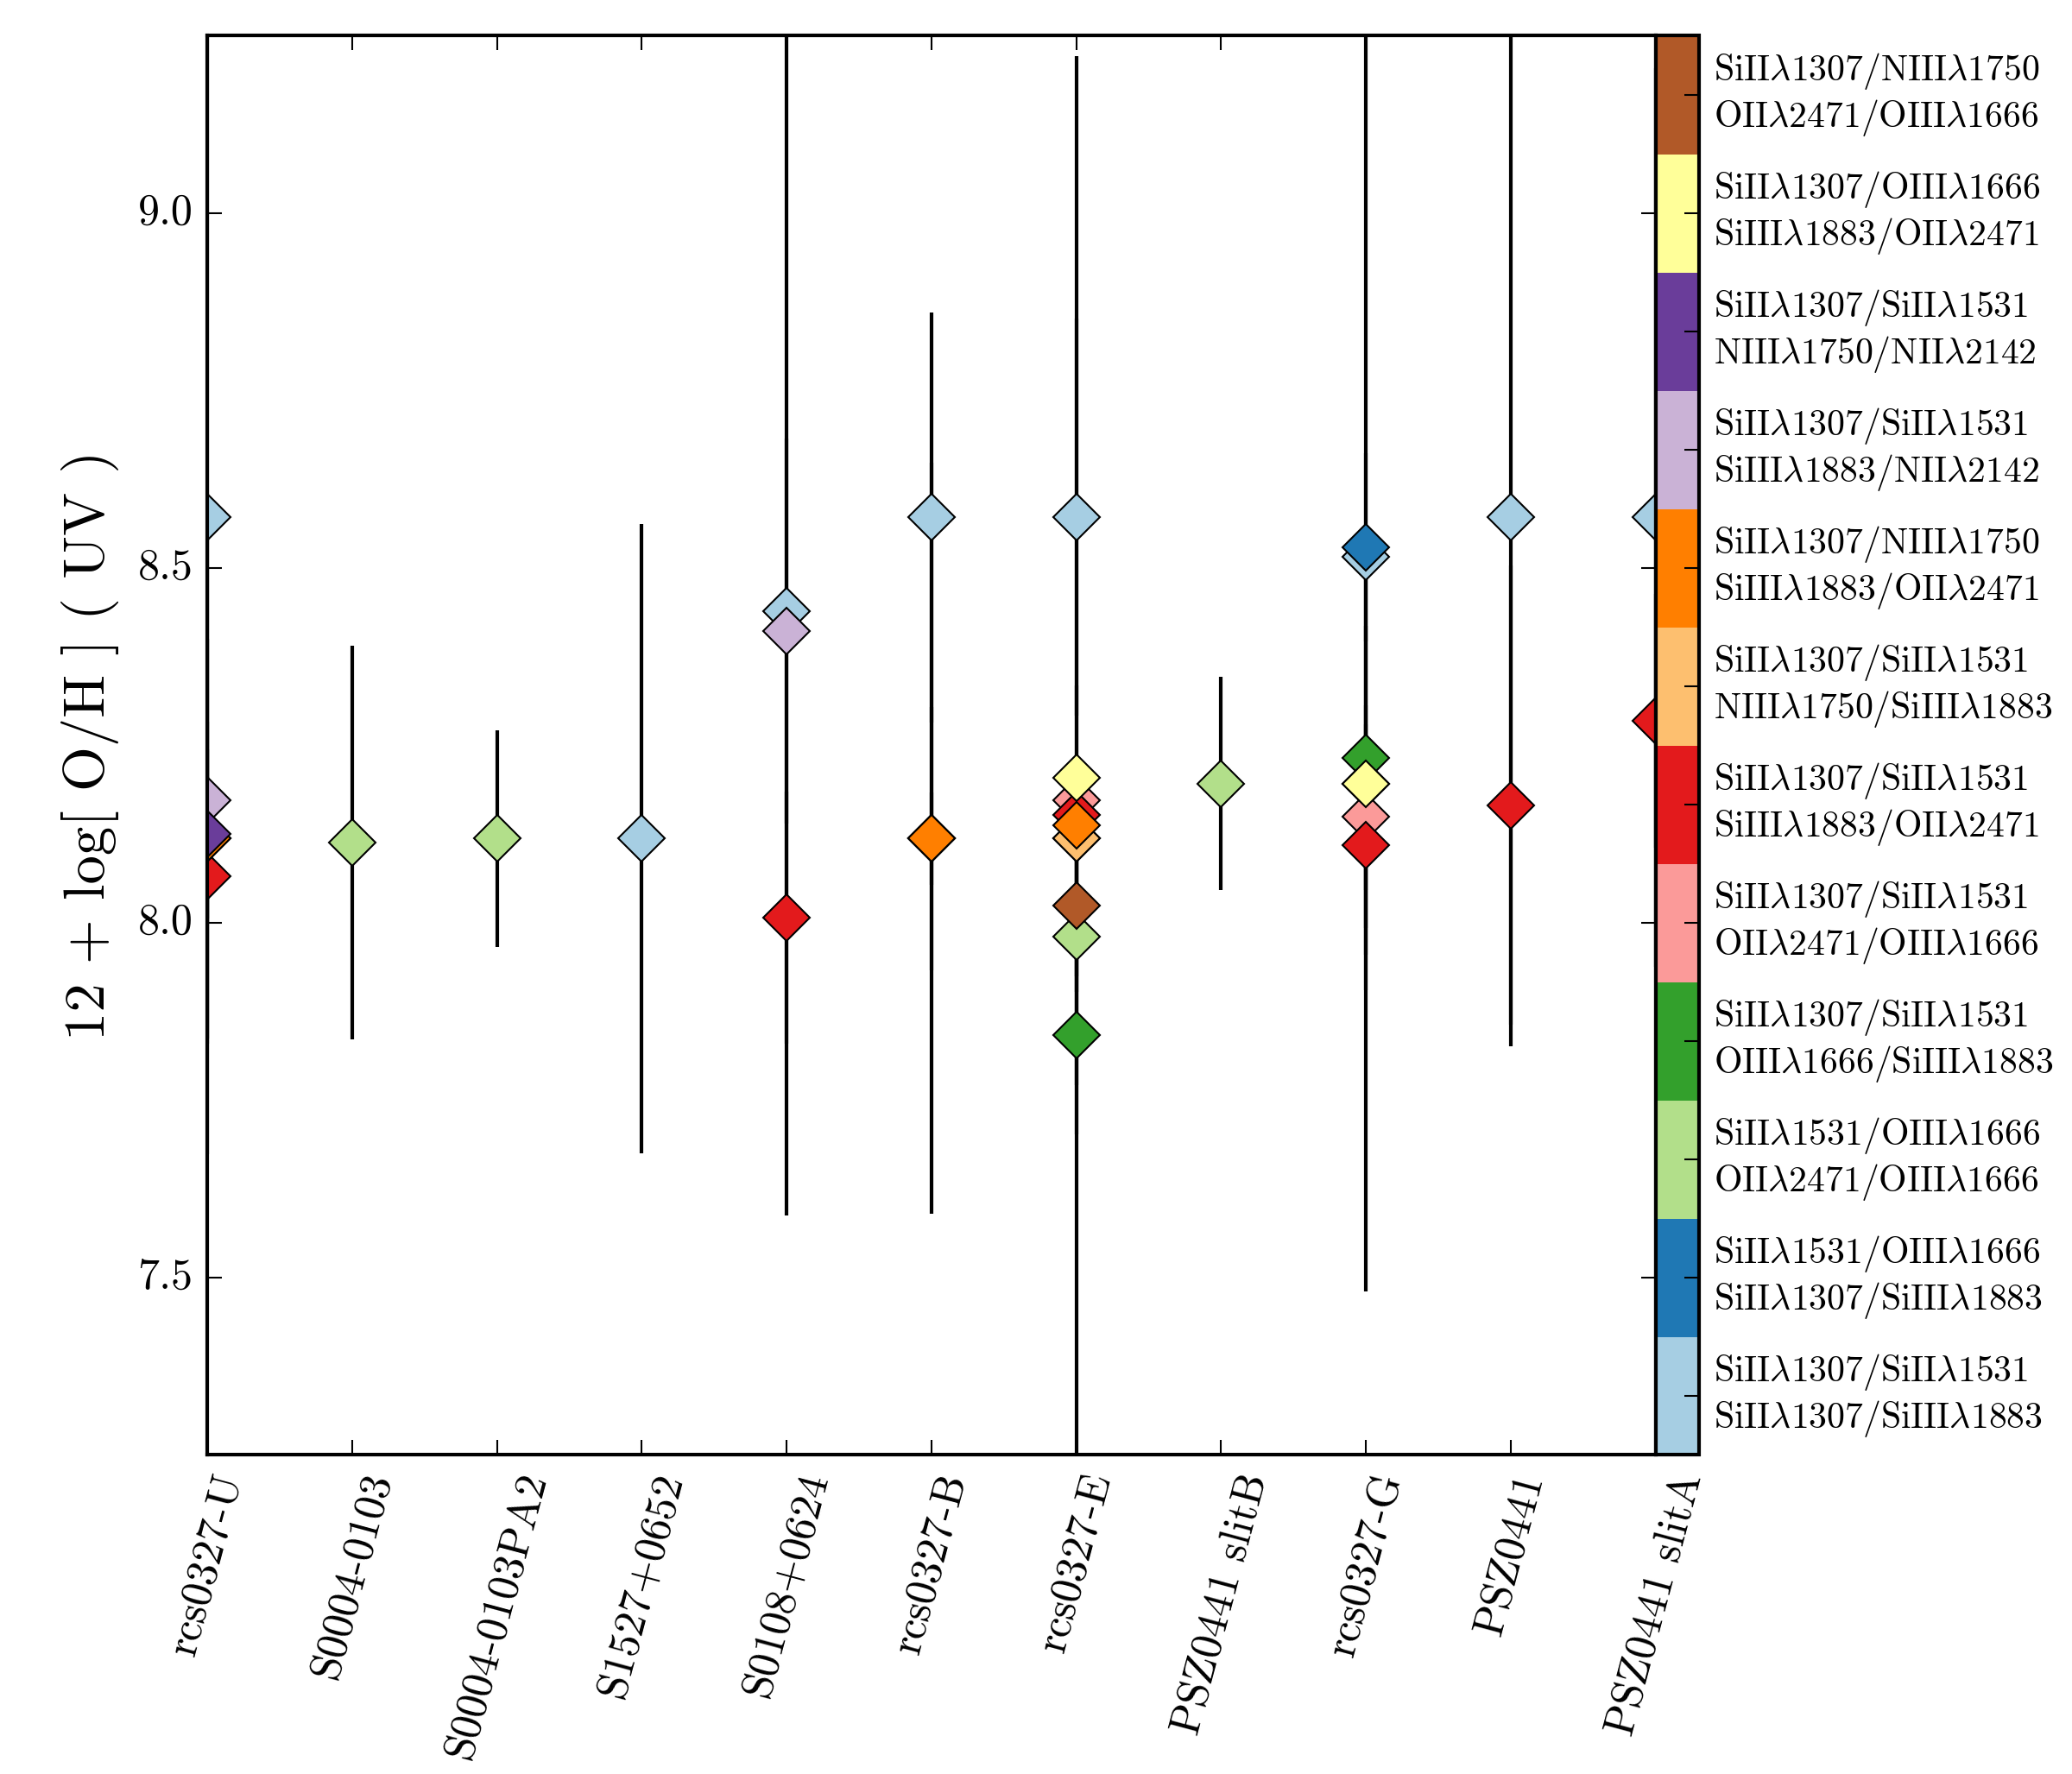
\includegraphics[width=\linewidth]{figs/f8.png}
    \caption{UV-derived metallicities ($y$-axis) for the \mage galaxies, each object is offset on the $x$-axis arbitrarily. Each marker is is color-coded by the diagnostic diagram used to derive the metallicity, as shown in the colorbar. }
    \label{fig:UVmage}
  \end{center}
\end{figure*}
%-------------------------------------------------------
\section{Caveats}\label{sec:caveats}

\section{Discussion}\label{sec:discussion}

In \S\ref{sec:UVOpt}, we found that that several of the UV diagnostics were poor metallicity indicators. Specifically, metallicities derived using diagnostics with \civ, \ciii, \SiuIII, and \heii were often inconsistent with optical metallicities, and, in some cases, completely uncorrelated with optical metallicities. In this section we briefly discuss possible explanations for the problematic behavior.

\subsection{Diagnostics with \ciii}

The UV Si3C3-O3C3 diagnostic diagram (Fig.~\ref{fig:UVSiO}) uses the \ciii$\lambda$1906,9 emission lines. Approximately 60\% of the metallicities derived with this diagnostic were consistent with the direct-\Te optical metallicity in the \citet{Berg+2016} sample of BCDs. However, the Si3C3-O3C3 diagnostic also predicted a much wider spread in metallicity than is found in the optical (1.2\,dex compared to 0.6\,dex). For several objects, the UV metallicity is entirely inconsistent with the optical metallicity, by several standard deviations.

We discuss two possible explanations for the inconsistencies between the UV and optical metallicities, including C/O ratio variations and nebular temperature fluctuations.

The \citet{Byler+2018} model uses a fixed relationship to describe the increase of [N/H] with [O/H] and [C/H] with [O/H] (\S\ref{sec:model:neb}). The relationship accounts for the additional production of N and C at high metallicity, and is matched to observations of local star-forming galaxies. It is important to note that these empirical relationships are used to describe the broad behavior of the galaxy population, and that individual objects can have an arbitrary abundance pattern for C,N, and O.

The C/O relationship used in this work was derived to match the \citet{Berg+2016} galaxies, and as such, most of the \citet{Berg+2016} galaxies have C/O ratios that are well-matched to our model. However, there are a handful of objects with C/O ratios that deviate significantly from our C/O relationship.

In the left panel of Fig.~\ref{fig:CO}, we again show the comparison between UV-derived metallicities with the direct-\Te optical metallicities for the \citet{Berg+2016} galaxies. Now, each point is color-coded by $\Delta$C/O, the deviation between the measured C/O ratio and the C/O ratio assumed by our model at that metallicity. Two of the objects where the UV-derived metallicity is systematically higher than the optical metallicity correspond to objects with C/O ratios that deviate significantly from the relationship used in this work.

It is thus possible that the \ciii line strengths are too sensitive to the specific C and O abundances to be a useful metallicity indicator. \citet{PerezMontero+2017} presented an analysis of metallicities derived using \ciii lines, and found that it was essential to estimate the C/O ratio before calculating the metallicity. We note that the C/O ratios of the two objects with over-estimated metallicities differ by nearly 0.4\,dex, and that there is little correlation between the C/O offset and the offset from the optical oxygen abundance.

Another possible explanation for the discrepant metallicities derived with the Si3C3-O3C3 diagnostic is the temperature sensitivity of the \ciii lines. The \ciii lines are known to be quite sensitive to temperature, and as relatively high ionization species, the \ciii lines will reflect conditions in the inner part of the nebula, where gas is closest to the ionizing source and temperatures are higher. Moreover, \citet{Dopita+1997} noted that these collisionally-excited lines should be a useful probe of shock-heated gas. Shock models predict stronger \ciii emission fluxes than either AGN or SF models.

In the right panel of Fig.~\ref{fig:CO}, we show the same UV-optical metallicity comparison, now color-coded by the \oiii electron temperature. The same two objects with overestimated metallicities and different C/O ratios have very similar temperatures, and the largest temperatures found in the \citet{Berg+2016} sample.

Hotter nebulae produce stronger \ciii emission, which would decrease both the Si3C3 and O3C3 ratios at fixed oxygen abundance, pushing objects toward higher metallicity models. We would expect the \ciii lines to be much more sensitive to the presence of shock heating than the optical \oiii lines, potentially explaining the overestimated metallicities from the Si3C3-O3C3 diagnostic. We plan to more thoroughly explore this explanation in future work.

%-------------------------------------------------------
% Figure 9:
%-------------------------------------------------------
\begin{figure*}
  \begin{center}
    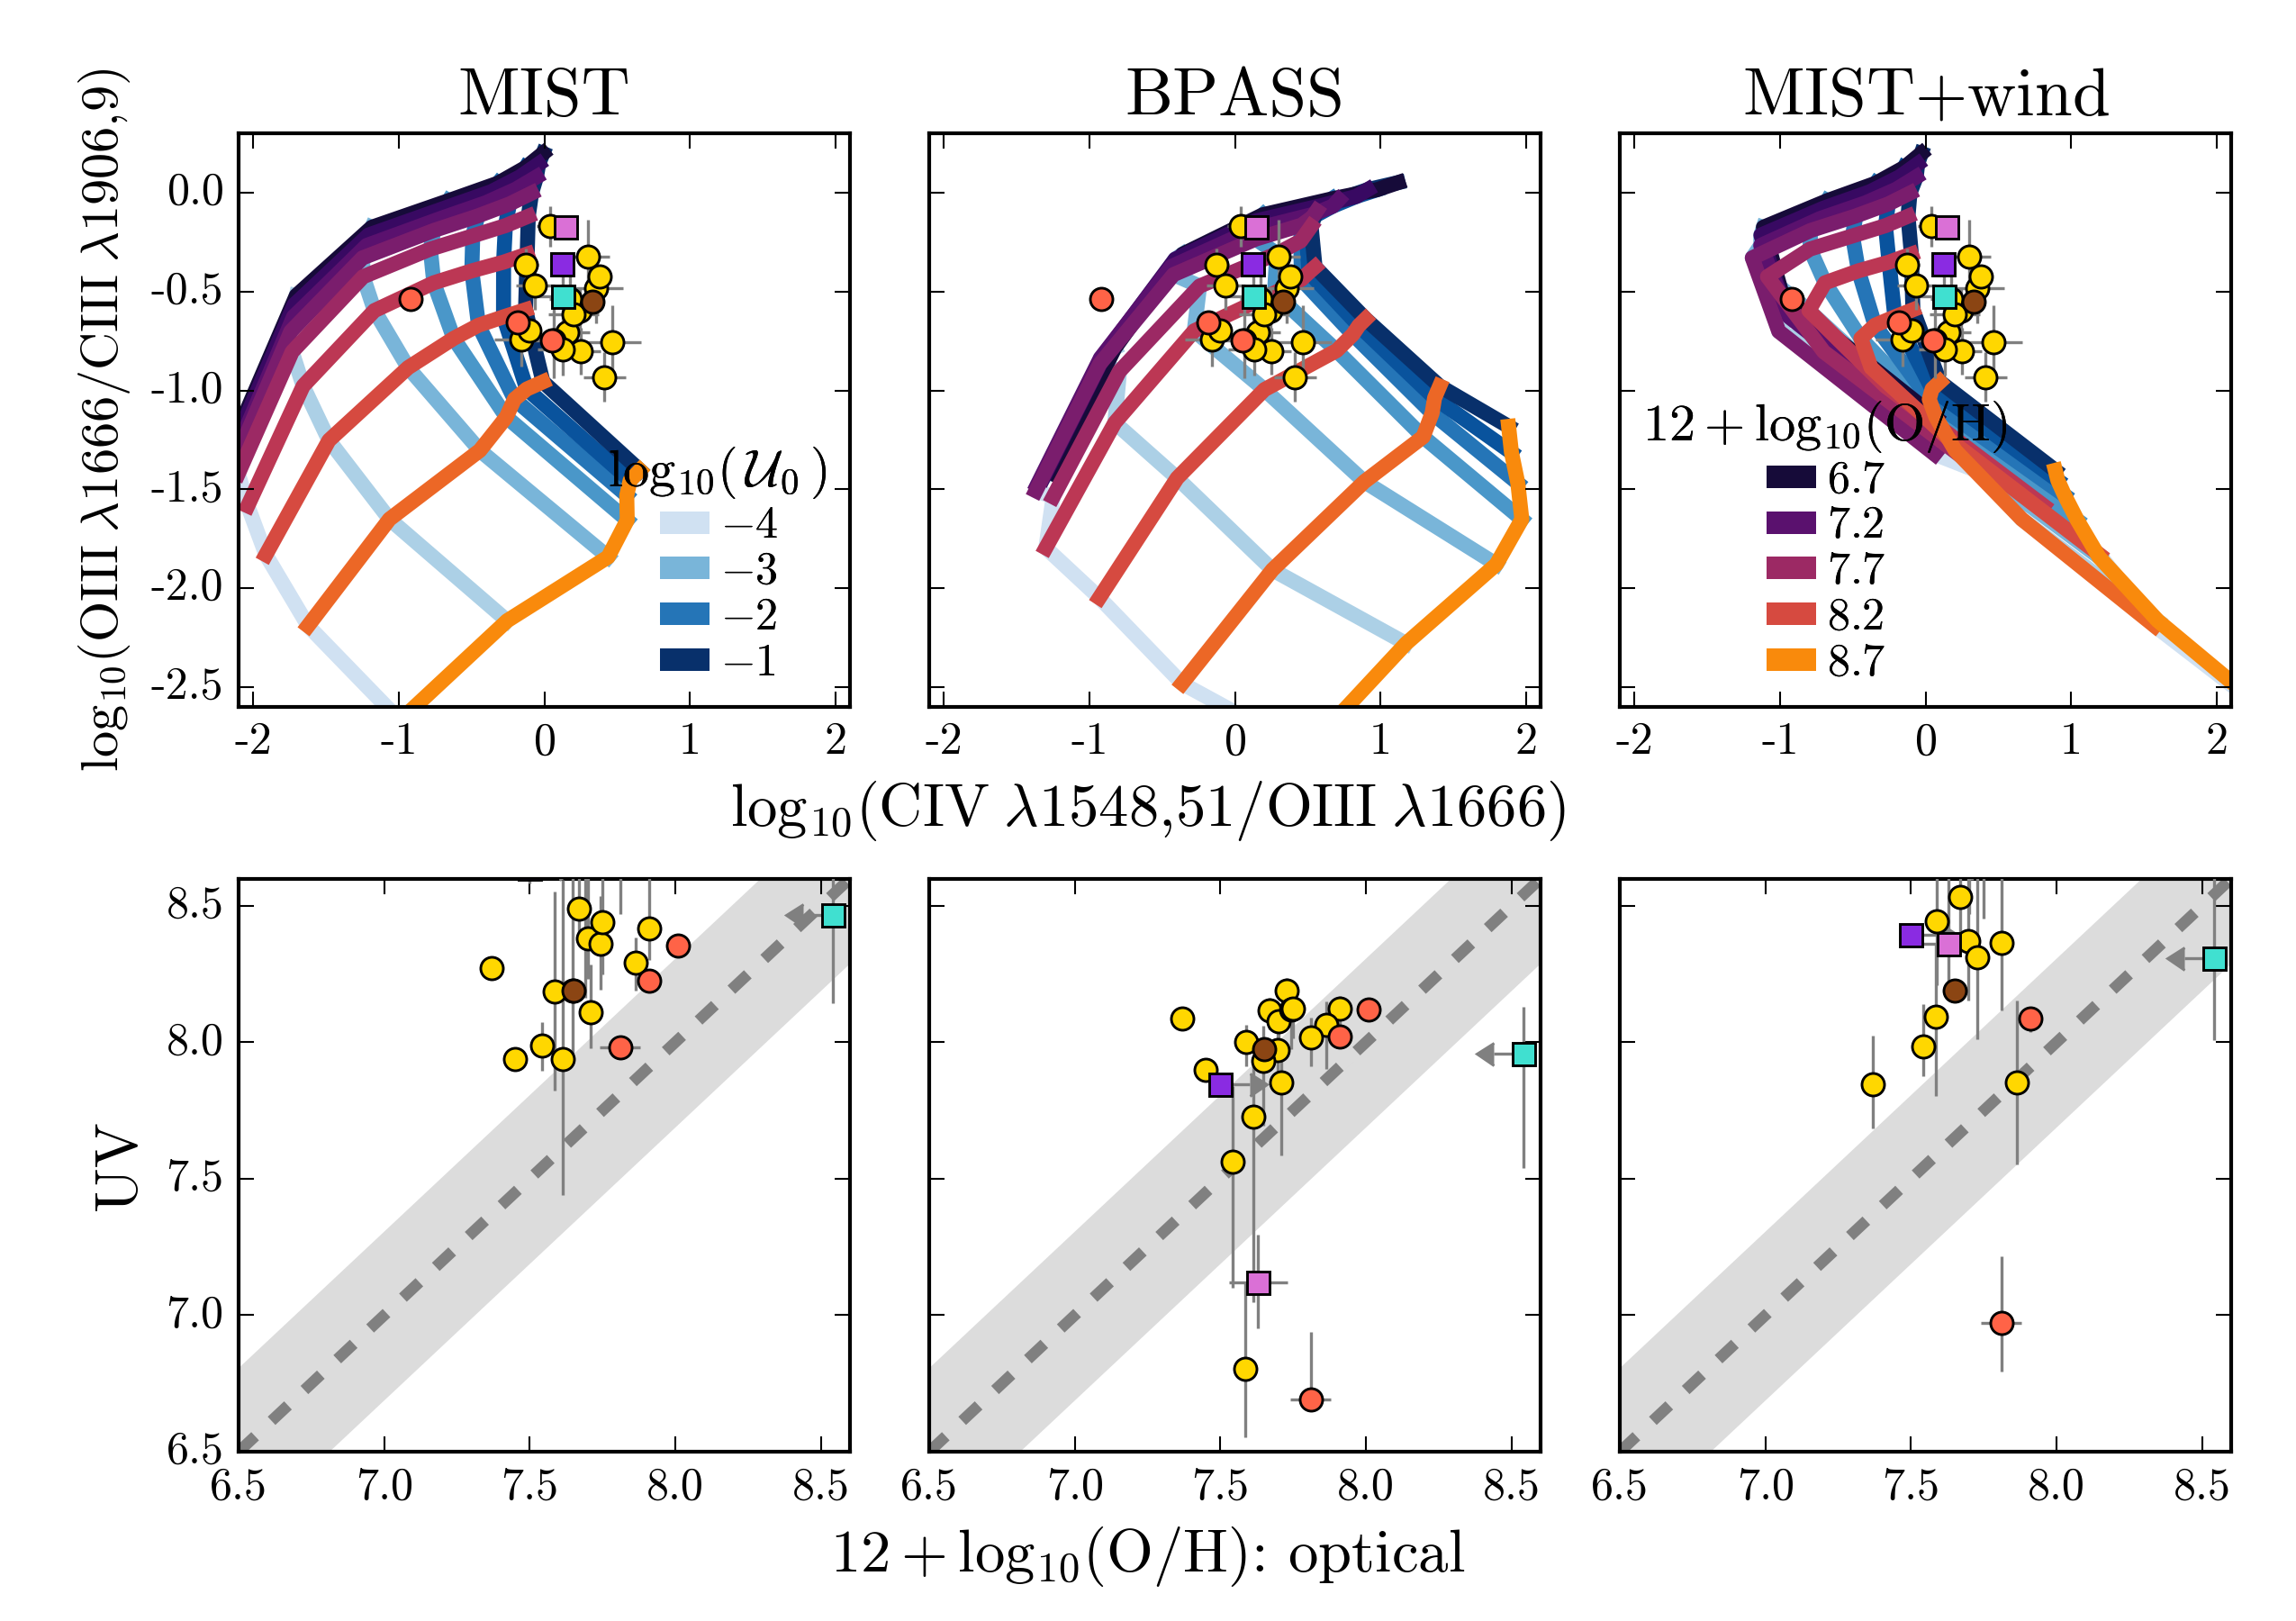
\includegraphics[width=\linewidth]{figs/f9.png}
    %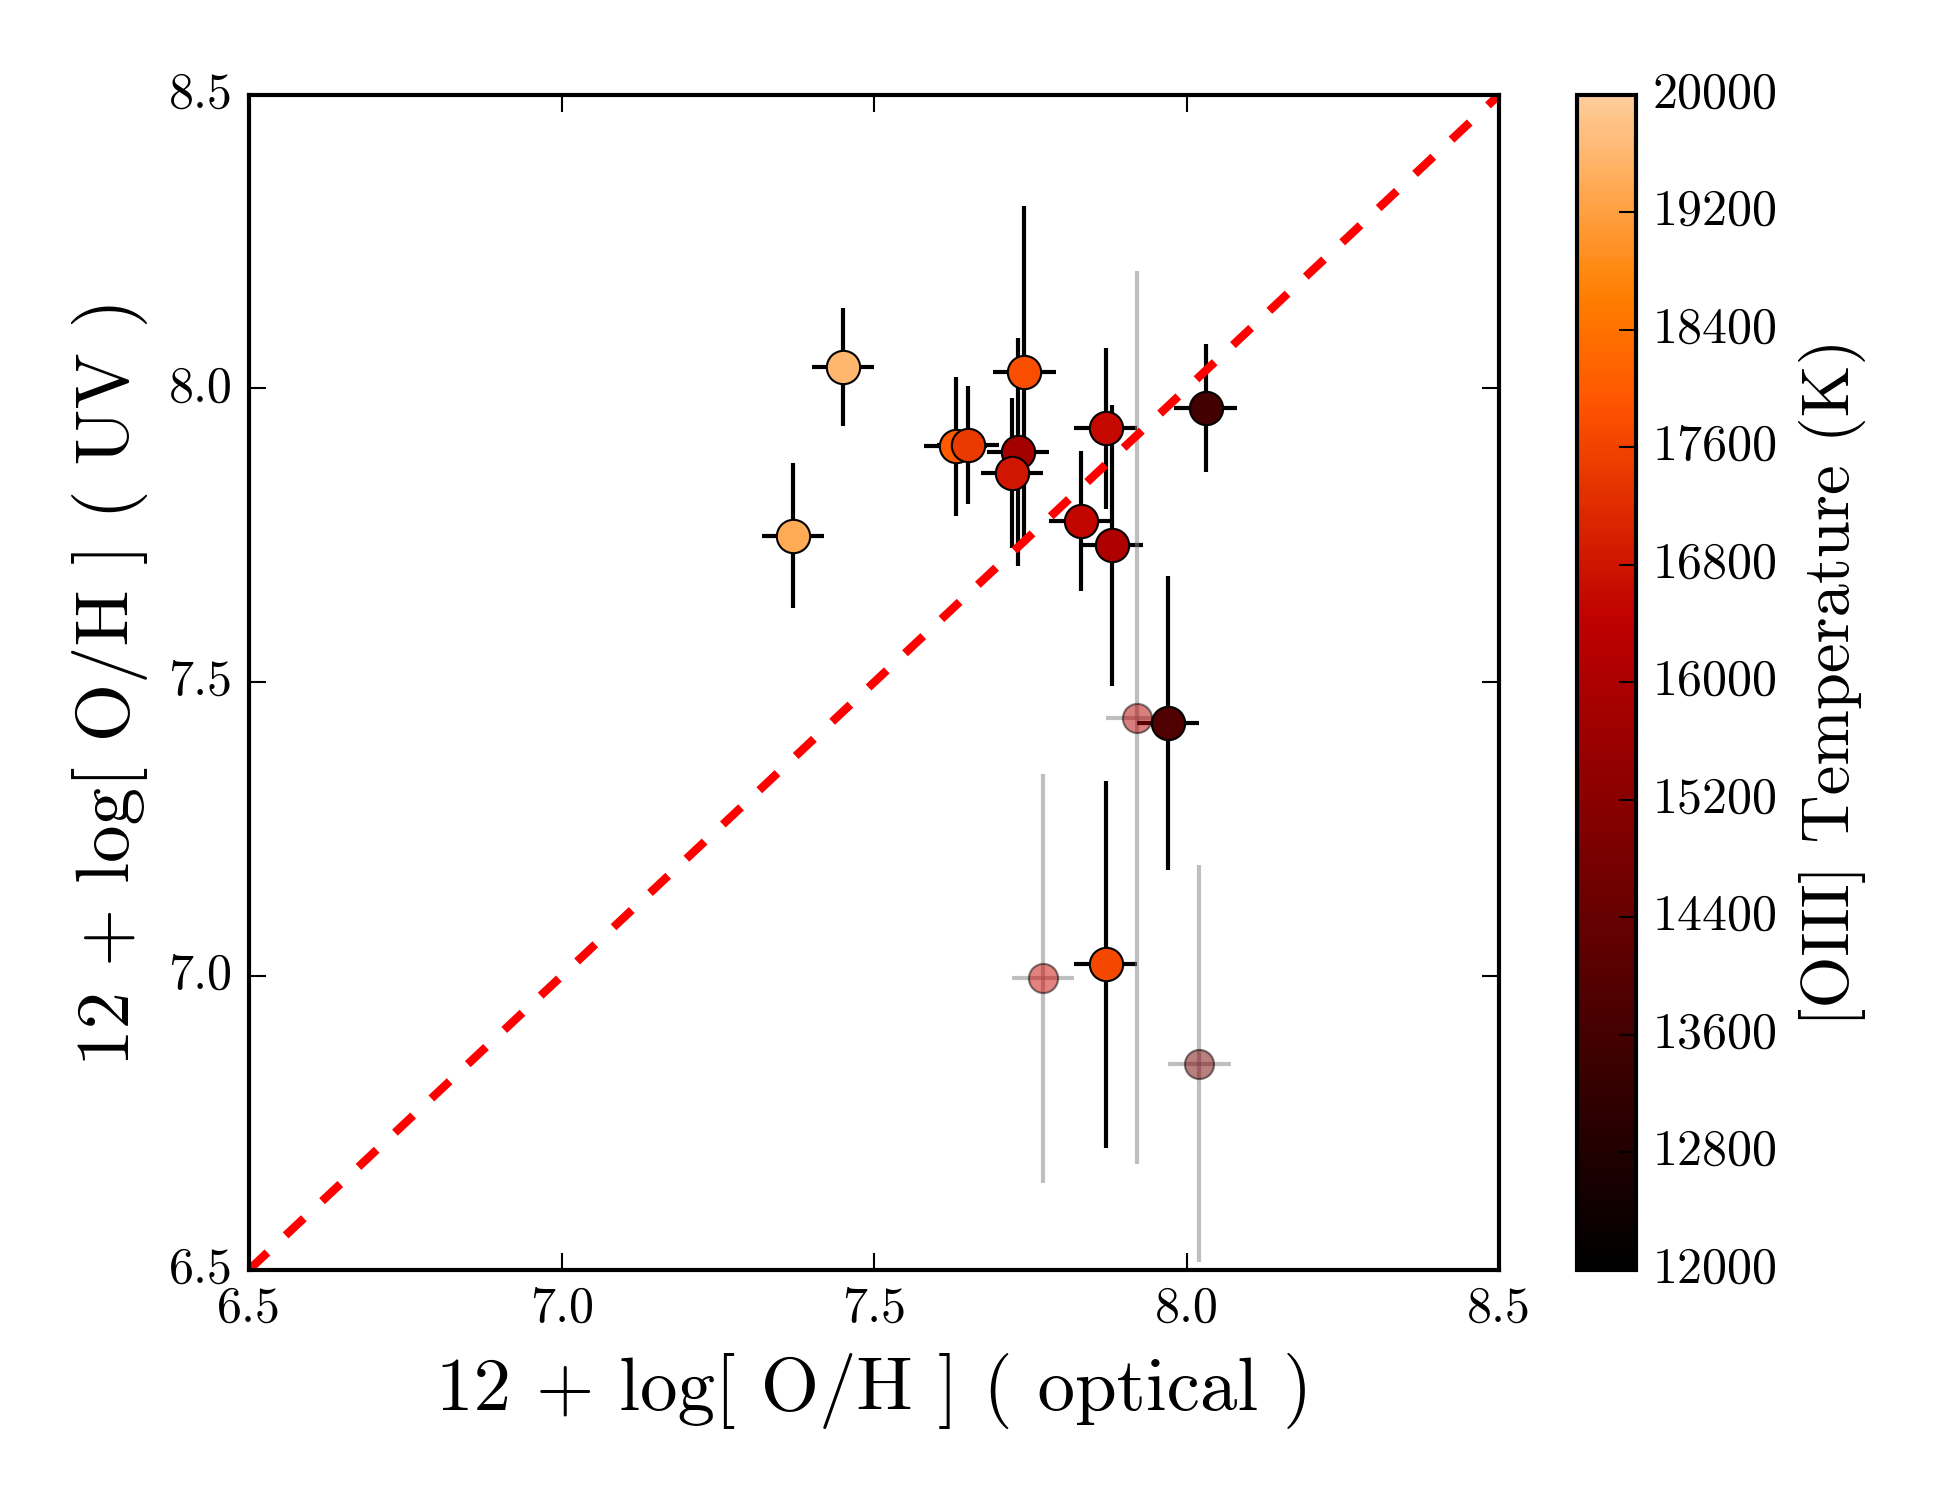
\includegraphics[width=0.45\linewidth]{figs/f8b.png}
    \caption{UV metallicities ($y$-axis) derived from the Si3C3-O3C3 diagnostic compared to the optical direct-temperature method oxygen abundance ($x$-axis) for the \citet{Berg+2016} galaxies. \emph{Left:} Objects are color-coded by the deviation between the measured C/O ratio and the C/O ratio assumed by the \citet{Byler+2018} model. \emph{Right:} Objects are color-coded by the electron temperature calculated using the \oiii emission lines. The \ciii emission lines should be sensitive to the presence of shock-heated gas, possibly explaining offset between UV and optical metallicities.}
    \label{fig:CO}
  \end{center}
\end{figure*}
%-------------------------------------------------------
\subsection{Diagnostics with \civ$\lambda$1550}

\civ emission is one of the more difficult spectral features to interpret, due to the competing effects of nebular emission at 1548 and 1550\ang, stellar wind emission at 1550\ang (often broad, with a strong P-Cygni profile) and interstellar absorption between 1540 and 1550\ang. Generally, the strength of the nebular \civ emission peaks at low metallicity ($12+\logOH \sim 7$) and high ionization parameter (\logU$>-2$). Stellar emission is wind-driven and strongest at higher metallicities, solar-like and above. However, even at $12+\logOH = 7.5$ (\logZ$\sim-1$), stellar \civ emission can account for as much as 30\% of the total \civ emission \citep{Byler+2018}.

Out of all the diagnostics presented in this work, the UV diagnostics that included the \civ$\lambda$1548,1550 lines preformed the worst, predicting metallicities that were systematically 0.2-0.6\,dex larger than optical metallicities. The \civ metallicities were inconsistent with optical metallicities in all objects, and showed only modest correlation with the optical metallicities.

We note that the \civ$\lambda$1548,1550 lines in the \citet{Berg+2016} spectra are in fact broader than the other nebular emission lines, which is consistent with wind contamination. Similarly, it makes sense that the \citet{Senchyna+2017} observations showed the best agreement with model emission line ratios and optical metallicity estimates, since the \civ fluxes in these objects were effectively ``nebular only''. However, even the \citet{Senchyna+2017} observations show a 0.1 - 0.3\,dex offset between the UV and optical metallicities, demonstrating the difficulty in using \civ as a metallicity diagnostic, especially at high redshift, where different gas conditions may prevail.

\subsection{Diagnostics with \heii$\lambda$1640}

The source of strong \heii emission in high redshift galaxies is a subject of open debate, and \heii emission is difficult to produce with current stellar models. We discuss two possible sources for \heii metallicity discrepancies: the use of ionizing spectra that are too soft and contamination from stellar wind emission.

Significant nebular \heii emission requires high energy photons, and current stellar models have difficulty producing the hard ionizing spectra required without invoking binary populations or rotating stars \citep[e.g.,][]{Stark+2014, Steidel+2016, Byler+2017}. Harder ionizing spectra would produce stronger \heii emission and create an extended partial ionization zone in the nebula, changing emission line ratios. More detailed modelling is required to understand if this could explain the discrepant metallicities.

\heii emission can also be produced in the winds of hot stars, which can be difficult to disentangle from the nebular emission without high resolution spectra. Current research suggests that only extreme, Wolf-Rayet (WR)-like stars should produce significant amounts \heii wind emission. These stars are short-lived and we do not expect them to dominate the \heii emission in all but extremely young star bursts.

Despite these complications, the He2C3 - O3C3 yielded metallicity measurements that agreed quite well with those in the optical, especially at low metallicities ($12+\logOH \lesssim 8$) where we expect broad \heii emission to be less prevalent. The worst agreement was found with the \mage galaxies, where the UV predicted lower metallicities than the optical by 0.5-1.0\,dex. However, visual inspection of the \heii spectral features in these objects revealed broad line profiles, indicating that stellar contamination may be responsible for the mismatch between UV and optical metallicities.

\subsection{Diagnostics with \SiuII, \SiuIII}

\XXX{FINISH HERE}:

Silicon emission lines proved to be fairly unreliable metallicity tracers.
Metallicity diagnostics that involve silicon lines tend to overestimate the metallicity, by as much as 1\dex in extreme cases. There are a few possible explanations for the mismatch between observed and model-predicted silicon line ratios, including: (1) incorrect silicon abundances (both the total gas phase abundance and the fraction depleted onto dust grains), (2) incorrect atomic data, (3) the sensitivity of the silicon ionization energy to age and metallicity variations in ionizing flux, and (4) possible contamination from supernovae (SNe) emission. We briefly discuss each of these explanations in turn.

The chemical composition of dust can evolve as grains lose atoms to the gas phase through high energy processes that occur in the supernova-generated shock waves in the ISM. High energy collisions between grains can cause erosion on the surface of dust, transferring elements (in particular Mg, Si, and Fe) from the grain surface to the gas phase. Notably, the fraction of silicon that is transferred back to the gas phase \emph{increases} with shock velocity \citep[see review on depletion patterns and dust evolution in][]{Jones+2000}.

shock velocity increases an increasing fraction of the
dust forming elements is transfered to the gas phase

Potentially: \citep{Jones+2000, Sankrit+2007, Okada+2008, Giannini+2015, Haris+2016}
Also: From \citet{Berg+2018} Our log(Si/O) measurement for SL2S0217 is remarkably consistent with this average from the Garnett et al. (1995a) study, but indicates significant Si/O enrichment or a reduced Si depletion onto dust relative to the z=2.4 galaxies of Steidel (2016).



%%%%%%%%%%%%%%%%%%%%%%%%%%%%%%%%%%%%%%%%%%%%%%%%%%%%%%%%%%%%%%%%%%%%%%%%%%%%%%%%
%===============================================================================
\section{Conclusions}\label{sec:conclusions}
%===============================================================================
\begin{enumerate}
    \item We have confirmed that UV and optical direct-temperature oxygen abundances agree within 0.1-0.2dex. The UV direct-\Te abundances are systematically lower than the optical-\Te abundances by 0.1 dex, which increases to a 0.2\,dex offset at solar and super-solar metallicities.
    \item UV metallicity diagnostics that include the \ciii$\lambda$1906,1909 emission lines do not reliably correlate with optical metallicities. We suggest that this is likely driven the presence of shock heated gas in addition to variations in C/O at fixed oxygen abundance.
    \item UV diagnostics that include the \civ$\lambda$1548,1550 emission lines are unreliable metallicity indicators. We suggest that this is primarily driven by the contamination from stellar emission, though interpretation is further complicated by strong interstellar absorption just blueward of the emission feature.
    \item UV diagnostics that include the \heii$\lambda$1640 emission line are reliable metallicity indicators at metallicities below $12+\logOH \sim 8$. At higher metallicities ($12+\logOH \sim 8.5$), discrepant abundances likely arise from contamination by stellar \heii emission.
    \item UV diagnostics that consist of ratios of silicon, oxygen, and nitrogen emission lines spanning multiple ionization states provide the most reliable metallicity estimates, like \SiuII$\lambda$1307/\SiuII$\lambda$1531 \vs \oiii$\lambda$1666/\SiuIII$\lambda$1883. Other promising diagnostics include \SiuII$\lambda$1307/\oiii$\lambda$1666 \vs \SiuIII$\lambda$1883/\oii$\lambda$2471, \SiuII$\lambda$1307/\SiuII$\lambda$1531 \vs \niii$\lambda$1750/\SiuIII$\lambda$1883, and \SiuII$\lambda$1307/\SiuII$\lambda$1531 \vs \oii$\lambda$2471/\oiii$\lambda$1666.
    \item Using the \mage galaxy sample, we demonstrate that metallicities derived using the above diagnostics are consistent with optical metallicities derived using empirically calculated strong line indices. Additionally, the metallicities derived using these diagnostics are consistent with metallicities derived using other UV diagnostics.
    \item We have calculated UV metallicities for the \mage galaxies using a weighted average of the five diagnostics presented above.
\end{enumerate}


%%%%%%%%%%%%%%%%%%%%%%%%%%%%%%%%%%%%%%%%%%%%%%%%%%%%%%%%%%%%%%%%%%%%%%%%%%%%%%%%
%-------------------------------------------------------
\bibliographystyle{aasjournal}
\bibliography{main}
%-------------------------------------------------------
\end{document}
